% Copyright 2004 by Till Tantau <tantau@users.sourceforge.net>.
%
% In principle, this file can be redistributed and/or modified under
% the terms of the GNU Public License, version 2.
%
% However, this file is supposed to be a template to be modified
% for your own needs. For this reason, if you use this file as a
% template and not specifically distribute it as part of a another
% package/program, I grant the extra permission to freely copy and
% modify this file as you see fit and even to delete this copyright
% notice. 

\documentclass{beamer}

% There are many different themes available for Beamer. A comprehensive
% list with examples is given here:
% http://deic.uab.es/~iblanes/beamer_gallery/index_by_theme.html
% You can uncomment the themes below if you would like to use a different
% one:
%\usetheme{AnnArbor}
%\usetheme{Antibes}
%\usetheme{Bergen}
%\usetheme{Berkeley}
%\usetheme{Berlin}
%\usetheme{Boadilla}
%\usetheme{boxes}
%\usetheme{CambridgeUS}
%\usetheme{Copenhagen}
%\usetheme{Darmstadt}
%\usetheme{default}
%\usetheme{Frankfurt}
%\usetheme{Goettingen}
%\usetheme{Hannover}
%\usetheme{Ilmenau}
%\usetheme{JuanLesPins}
%\usetheme{Luebeck}
%\usetheme{Madrid}
%\usetheme{Malmoe}
%\usetheme{Marburg}
%\usetheme{Montpellier}
%\usetheme{PaloAlto}
%\usetheme{Pittsburgh}
%\usetheme{Rochester}
%\usetheme{Singapore}
%\usetheme{Szeged}
%\usetheme{Warsaw}

\usepackage{amsmath}
\usepackage{textpos}
\usepackage{ulem}

\definecolor{BYUblue}{RGB}{0,31,69}
\definecolor{BYUgold}{RGB}{195,163,106}
\usecolortheme[RGB={0,31,69}]{structure} % BYU Blue

\definecolor{metric-PR}{RGB}{255,127,0}
\definecolor{metric-NE}{RGB}{51,51,255}
\definecolor{metric-OFI}{RGB}{204,0,0}
\definecolor{metric-IRO}{RGB}{0,204,0}

\usetheme{Frankfurt}
\setbeamercolor*{section in head/foot}{bg=BYUblue,fg=gray!25}
\setbeamercolor*{frametitle}{bg=BYUblue!50,fg=white!25}
\setbeamercovered{transparent}
\mode<all>

\DeclareMathOperator*{\argmax}{arg\,max}

\title{Informative Path Planning\\
with a Human Path Constraint}

%\subtitle{Optional Subtitle}

\author{Daqing Yi 
%\and Michael A. Goodrich \and Kevin D. Seppi
}


\institute
{
  Department of Computer Science\\
  Brigham Young University
}

\date[]{} 

\addtobeamertemplate{frametitle}{}{%
\begin{textblock*}{100mm}(0.9\textwidth,-1.2cm)

\includegraphics[width=1.1cm]{figure/BYU_logo.png}
\end{textblock*}}

\begin{document}

\begin{frame}
  \titlepage
\end{frame}

\begin{frame}{Outline}{Structure}
  \tableofcontents
  % You might wish to add the option [pausesections]
\end{frame}

% Section and subsections will appear in the presentation overview
% and table of contents.

\section{Introduction}

\begin{frame}{Modeling human intent}{Path Planning}
THe problem in modeling human intent
\begin{itemize}
\item incomparability in objectives
\item conflict in objectives
\item hardness in weighing the objectives
\item vagueness in importance selection
\end{itemize}
\begin{figure}
\centering
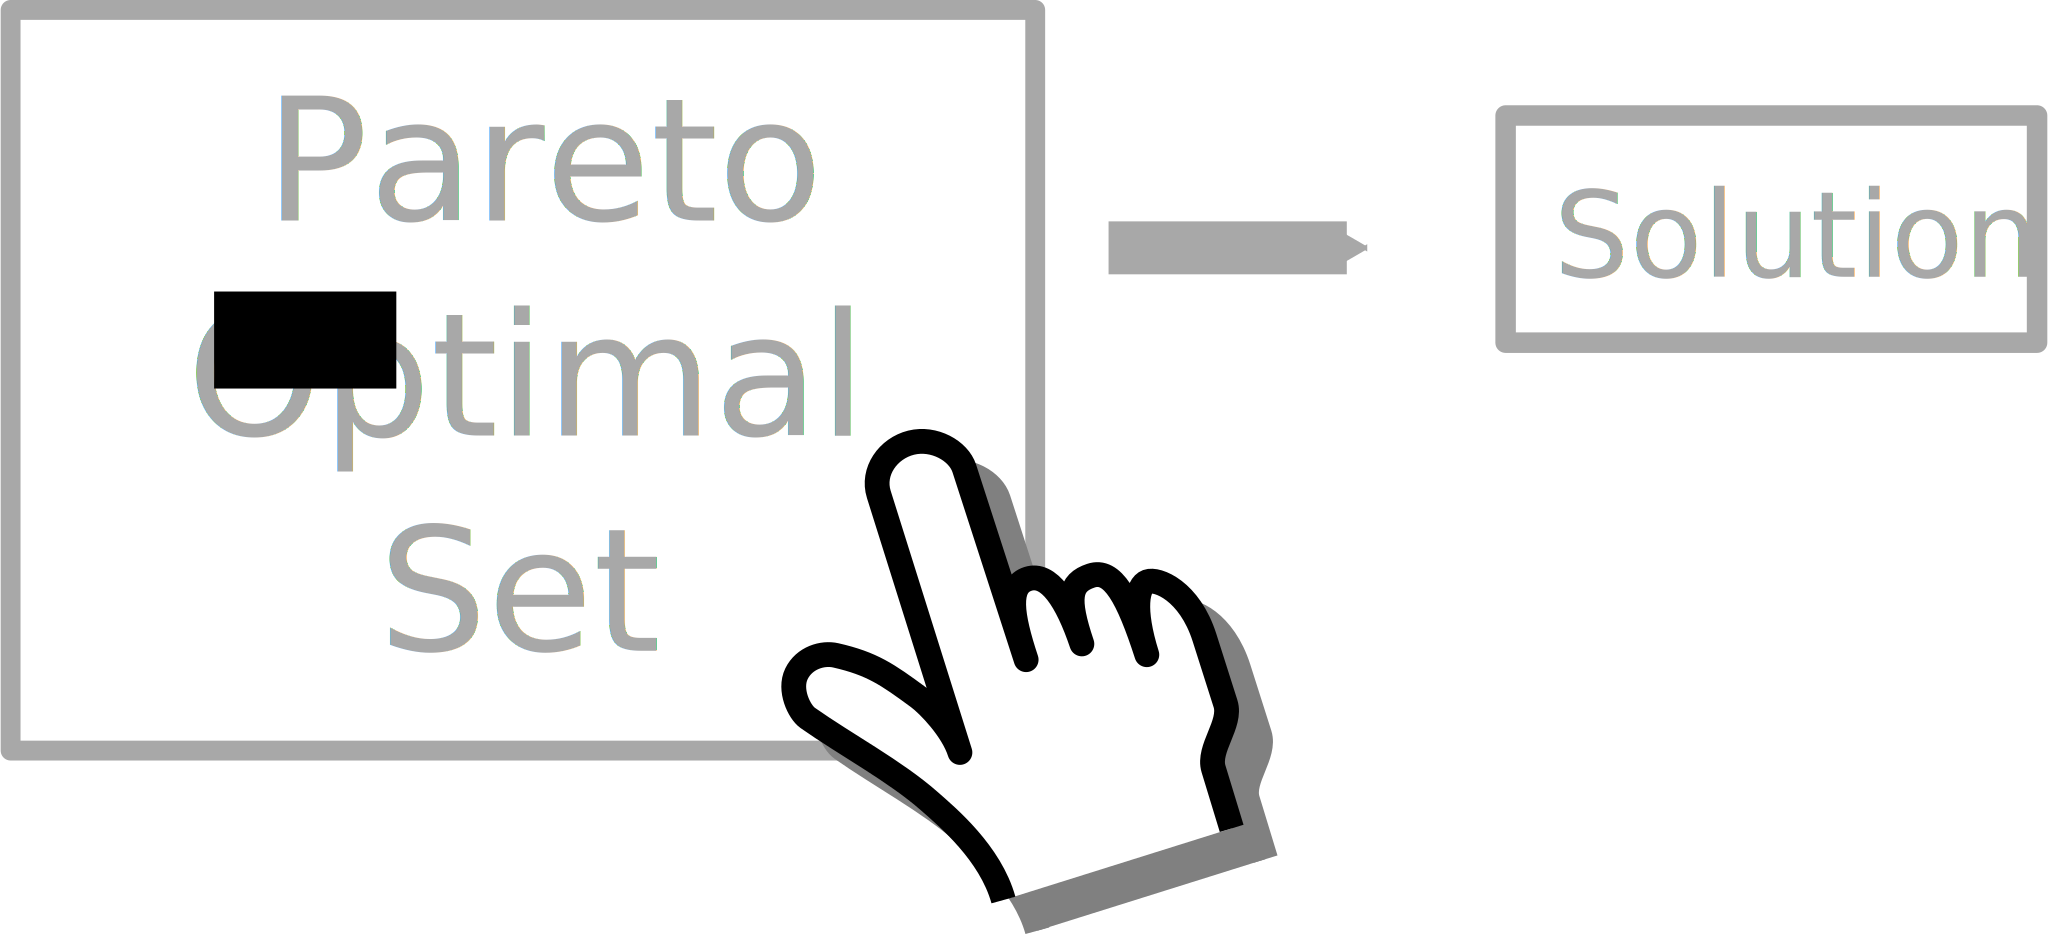
\includegraphics[width=0.6\linewidth]{figure/human_interactive_moo}
%\caption{}
\label{fig:human_interactive_moo}
\end{figure}
\end{frame}

\begin{frame}{Pareto Optimal}{}
\end{frame}

\section{Problem definition}

\subsection{Informative path}

\begin{frame}{Coverage model}{Informative path}

\begin{itemize}
\item Information measurement - entropy 
\item Maximum coverage problem
\end{itemize}

\begin{figure}
\centering
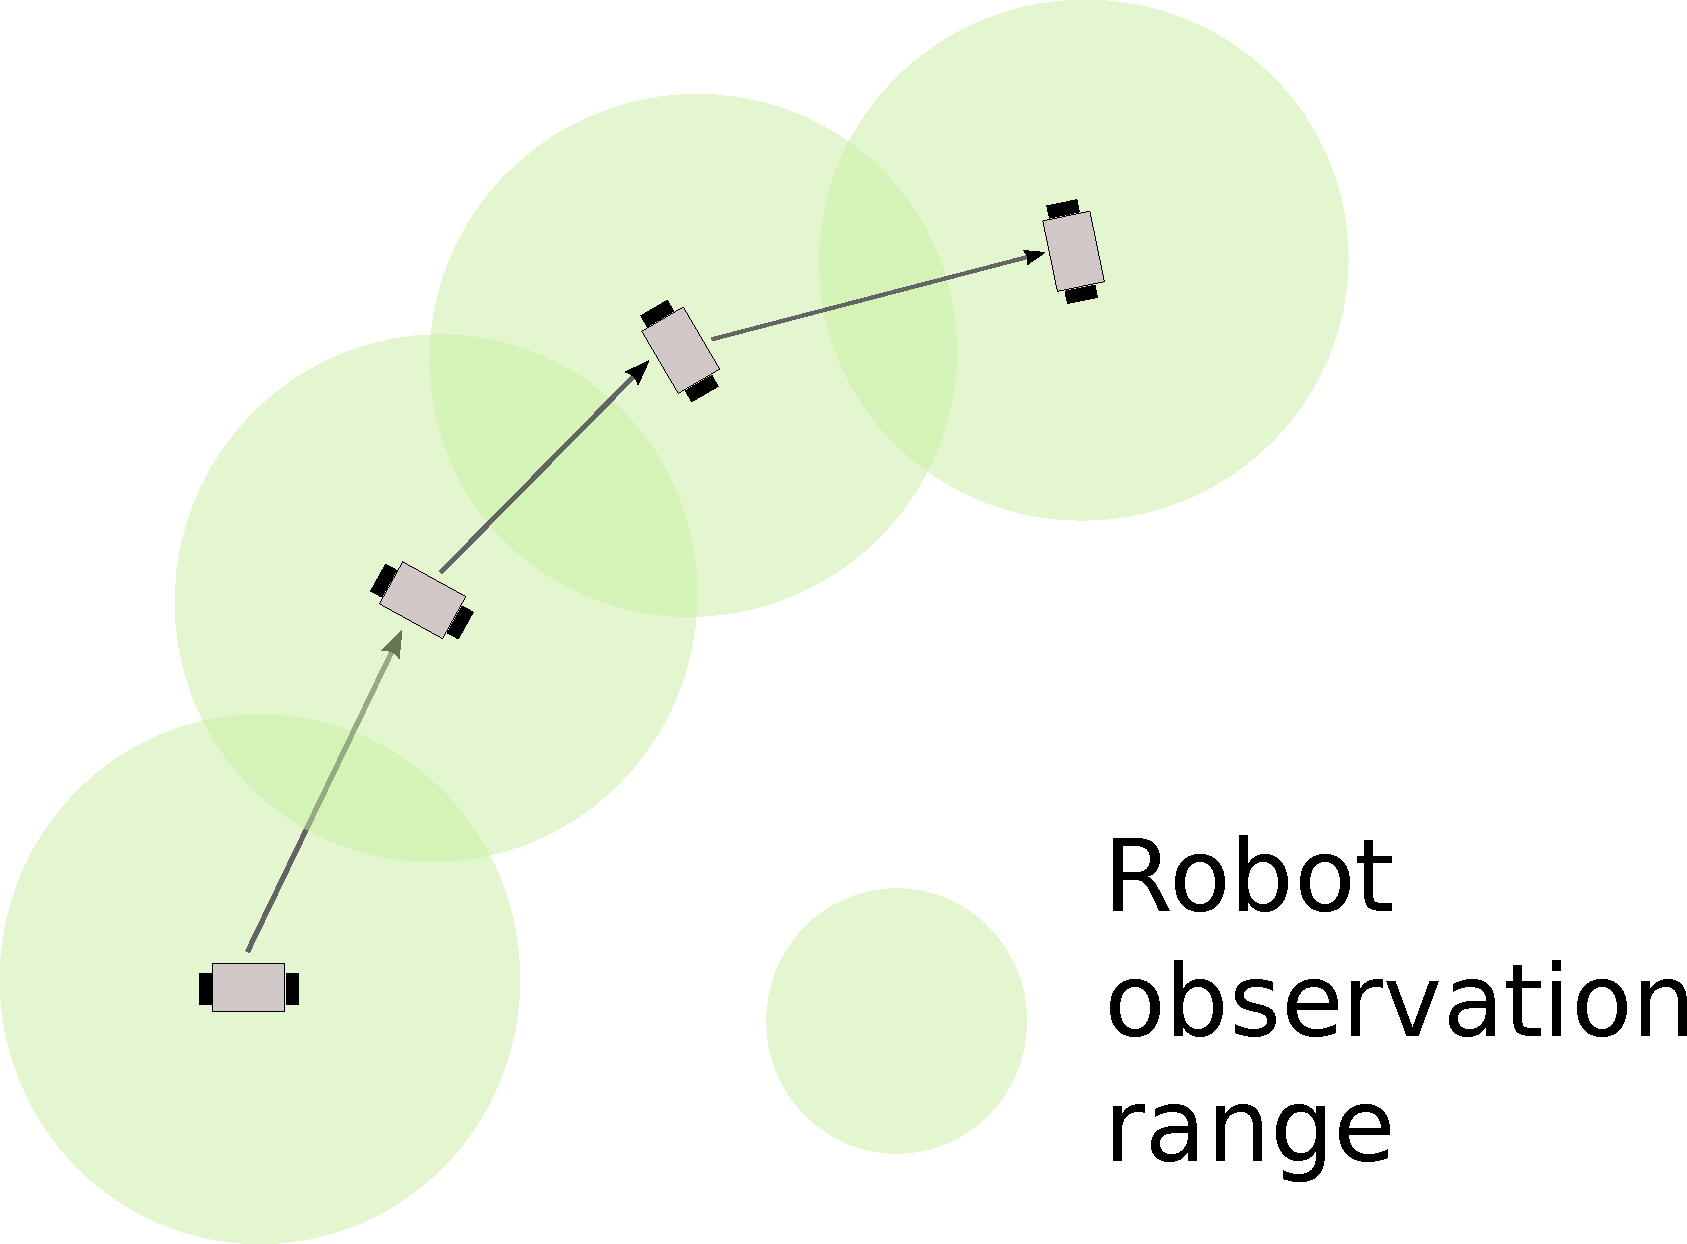
\includegraphics[width = 0.6\textwidth]{./figure/robotObservation}
%\caption{A coverage model.}
\end{figure}

\end{frame}

\begin{frame}{Submodularity}{Informative path}

\begin{columns}

\column{0.45\textwidth}

\begin{figure}
\centering
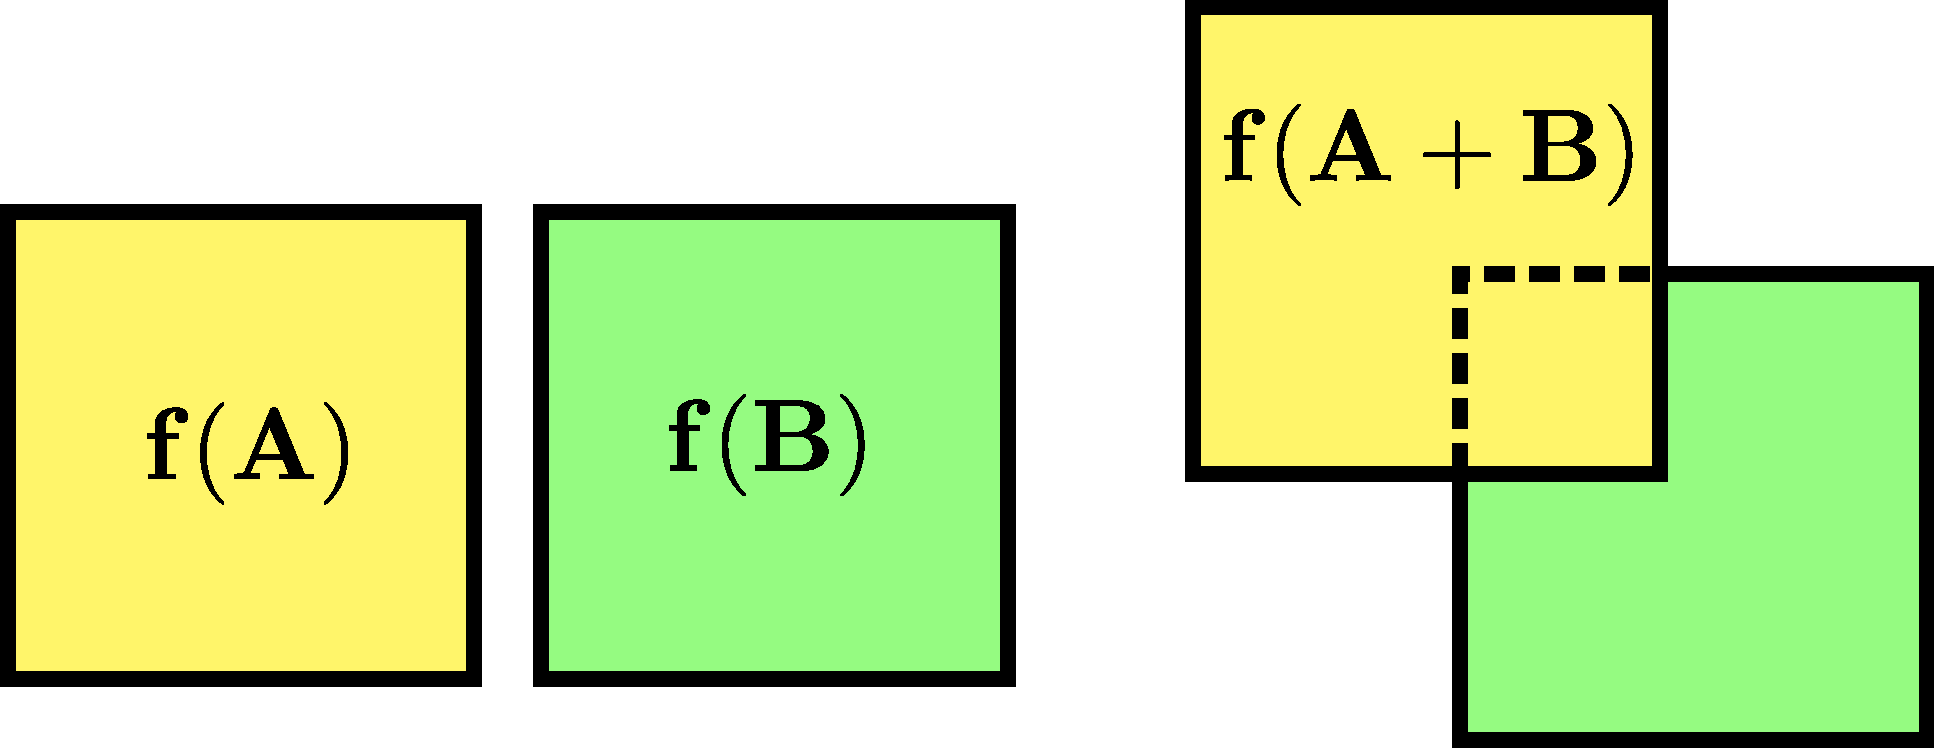
\includegraphics[width = \textwidth]{./figure/submodular}
%\caption{A coverage model.}
\end{figure}

\begin{equation}
\nonumber
f(A) + f(B) \geq f(A+B)
\end{equation}

\column{0.1\textwidth}

\column{0.45\textwidth}

Information
\begin{itemize}
\item search space $ S $
\item the observation of a robot $ \mathbf{O}^{X} $ 
\item the observation of a human $ \mathbf{O}^{Y} $

\bigskip
\bigskip

$ f( \mathbf{S}, \mathbf{O}^{X} ) + f( \mathbf{S}, \mathbf{O}^{Y^{h}} ) \geq f( \mathbf{S}, \mathbf{O}^{X},  \mathbf{O}^{Y^{h}} ) $ 
\end{itemize}

\end{columns}

\end{frame}

\begin{frame}{Submodular orienteering}{Informative path}

\begin{block}{Conditional mutual information}
$ I(\mathbf{S}; \mathbf{O}^{X} \mid \mathbf{O}^{Y^{h}}) = H(\mathbf{S} \mid \mathbf{O}^{Y^{h}}) - H(\mathbf{S} \mid \mathbf{O}^{X},\mathbf{O}^{Y^{h}}) $
\end{block} 

\bigskip

\begin{itemize}
\item Entropy reduction
\item Submodularity
\item Chain rule \\
$ I(\mathbf{S}; \mathbf{O}^{X} \mid \mathbf{O}^{Y^{h}}) = \sum_{t=1}^{T} I(O^{X}_{t} ; \mathbf{S} \mid O^{X}_{1} , \cdots , O^{X}_{t-1}, \mathbf{O}^{Y^{h}}) $
\end{itemize}

\end{frame}

\subsection{Human constraint}

\begin{frame}{Team role}{Human constraint}

\begin{figure}
\centering
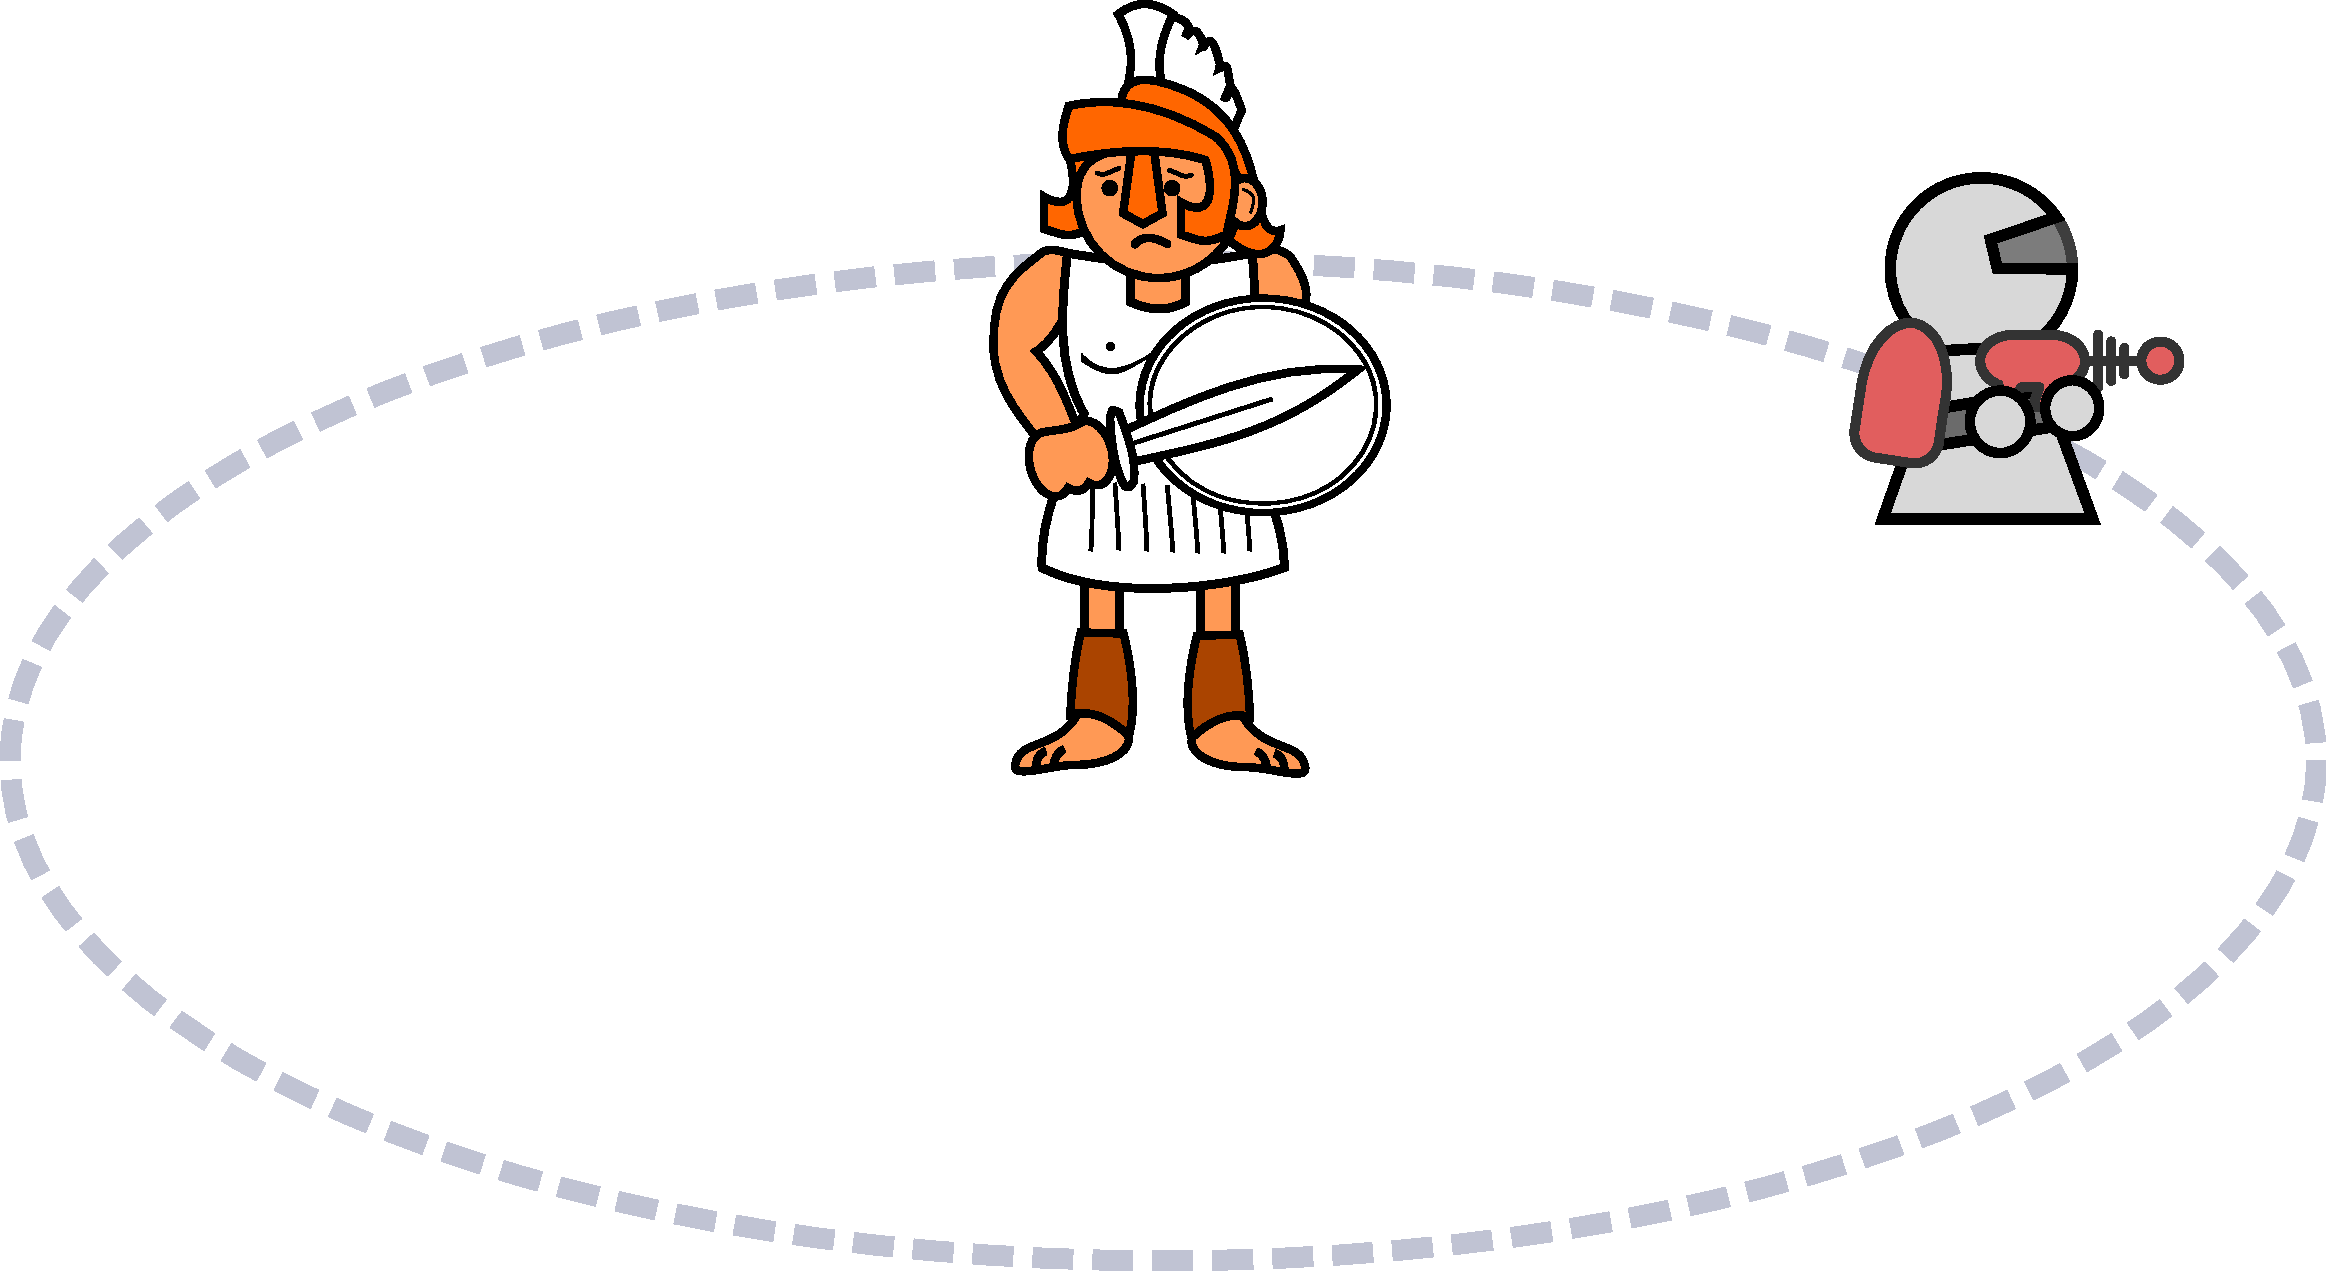
\includegraphics[width = 0.7\textwidth]{./figure/human_robot_interaction}
\end{figure}

\begin{itemize}
\item cooperative observation
\item assistance and protection
\end{itemize}

\end{frame}

\begin{frame}{Neighboring function}{Human constraint}

\begin{columns}
\column{.6\linewidth}
\begin{minipage}[c]{\linewidth}
\begin{figure}
\centering
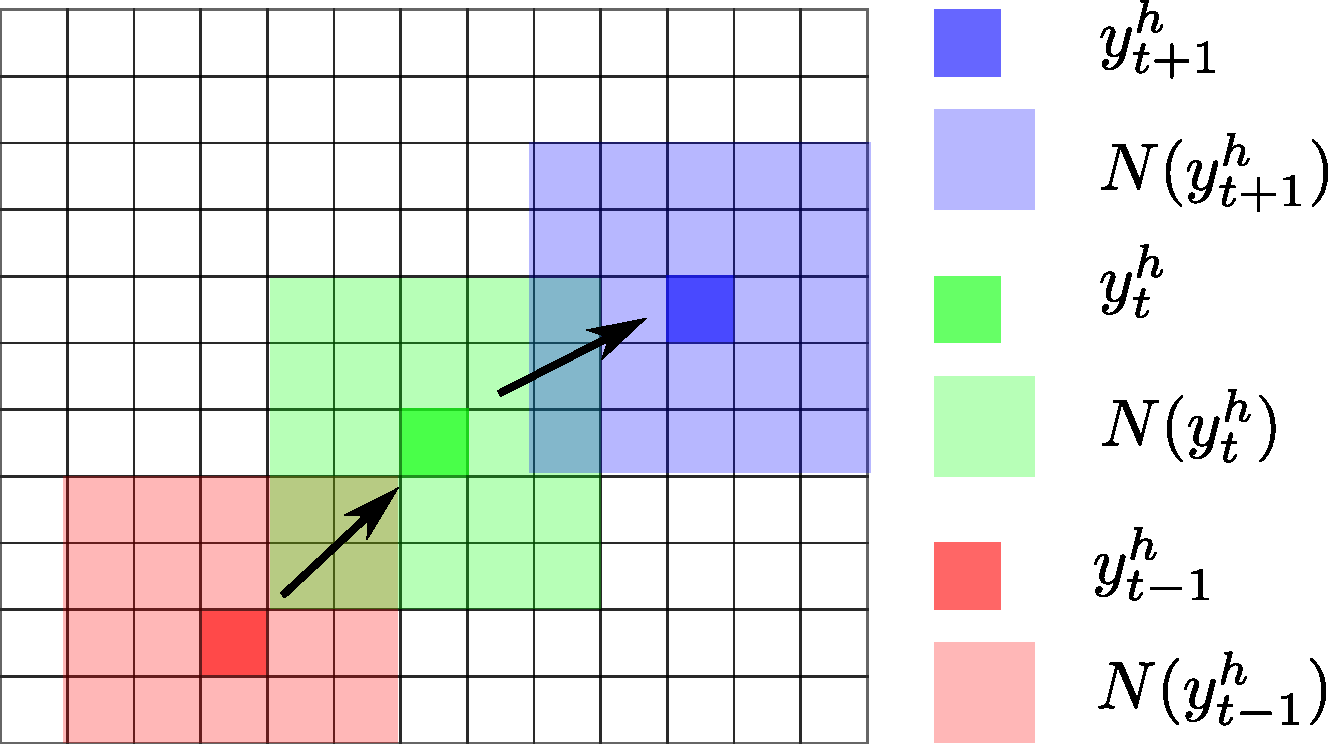
\includegraphics[width = \textwidth]{./figure/humanConstraint}
%\caption{An example of human constraint.}
\end{figure}
\end{minipage}

\column{.4\linewidth}
\begin{minipage}[c]{\linewidth}
\begin{itemize}
\item { human path $ \{ y^{h}_{1} \cdots y^{h}_{T} \} $ }
\item { neighboring function $ N( y^{h}_{t} ) $ }
\end{itemize}
\end{minipage}
\end{columns}

\end{frame}

\subsection{The optimization model}

\begin{frame}{Problem abstraction}{The optimization model}

\begin{figure}
\centering
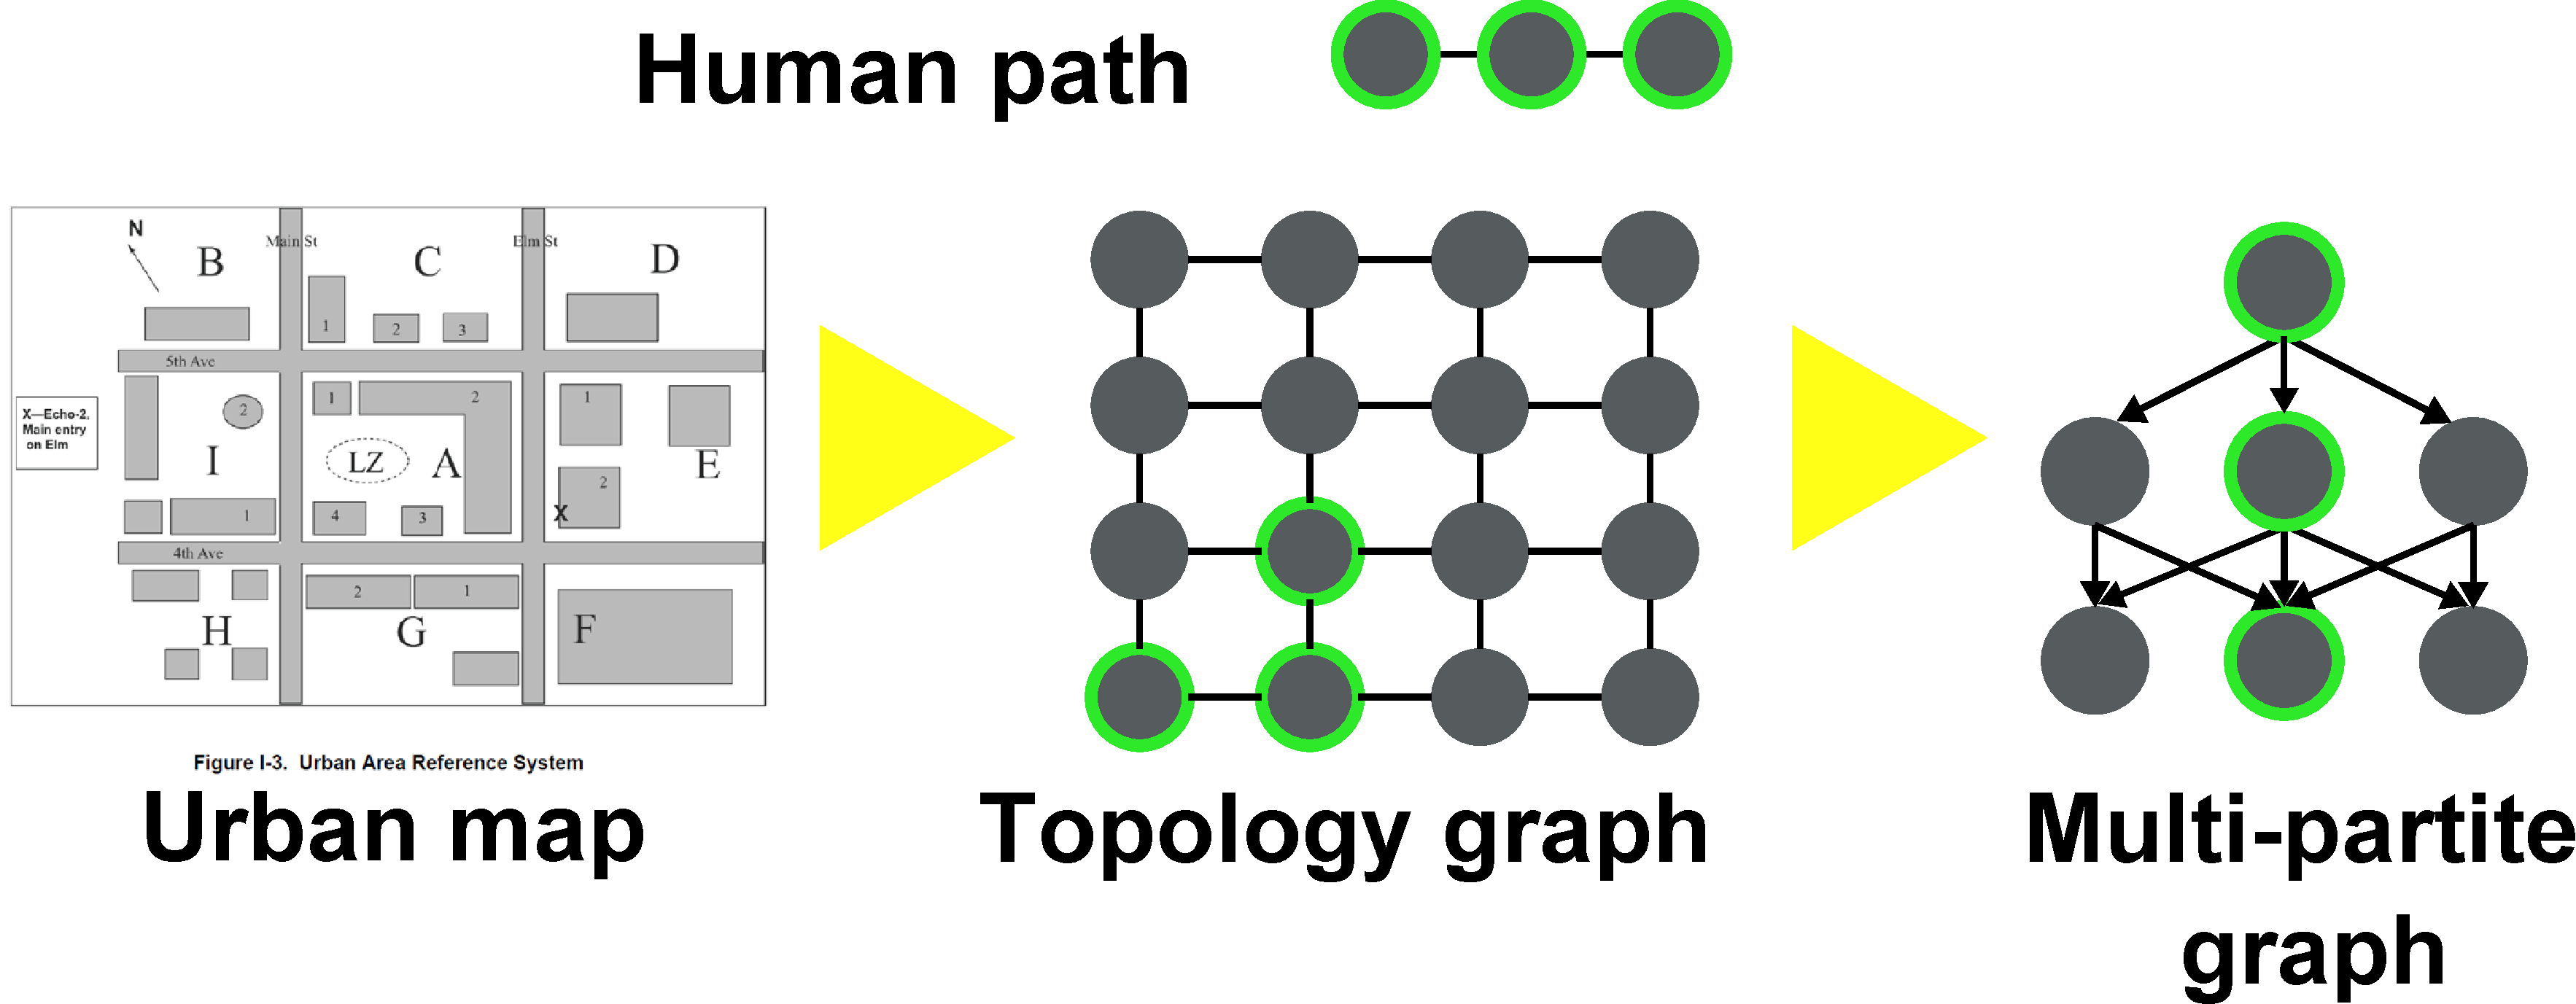
\includegraphics[width = 0.9\textwidth]{./figure/layers}
%\caption{A layered problem processing.}
\end{figure}

\end{frame}

\begin{frame}{The multi-partite graph}{The optimization model}

\begin{columns}

\column{.6\textwidth}
\begin{minipage}[c]{\textwidth}
\begin{figure}
\centering
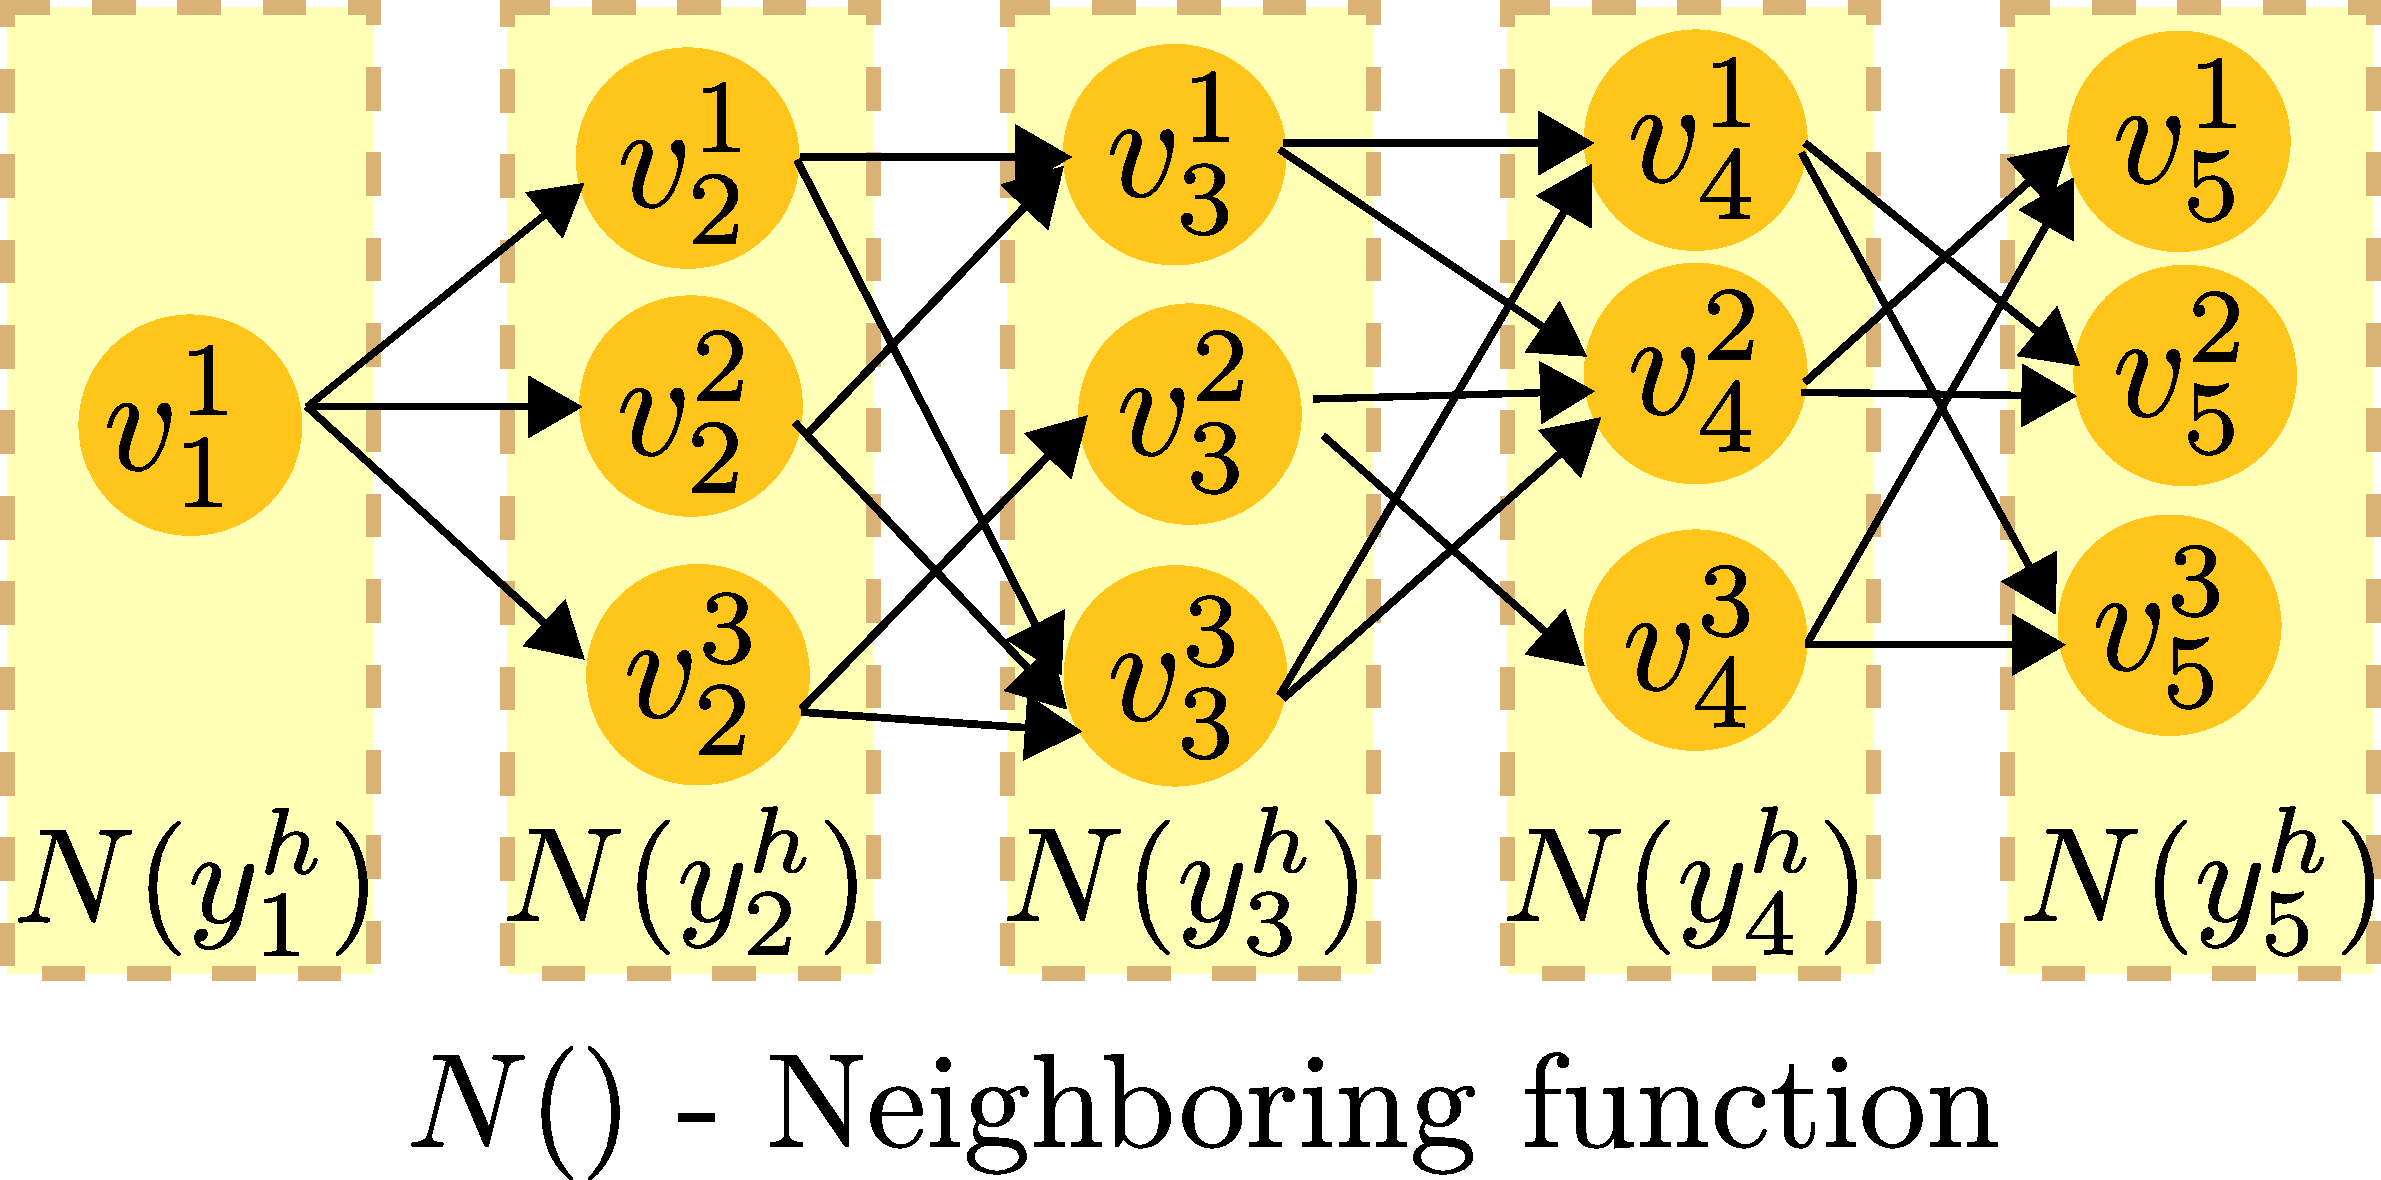
\includegraphics[width = \textwidth]{./figure/MultiPartite}
%\caption{A multi-partite graph generated from human constraint.}
\end{figure}
\end{minipage}

\column{.4\textwidth}
\begin{minipage}[c]{\textwidth}
\begin{itemize}
\item time-space synchronization
\item connection determined by discretized map
\end{itemize}
\end{minipage}

\end{columns}

\end{frame}

\begin{frame}{A pruning process}{The optimization model}

\begin{columns}
\column{.45\textwidth}
%\begin{minipage}
%\begin{block}
Reachable
%\end{block}
%\end{minipage}

\column{.45\textwidth}
%\begin{minipage}
%\begin{block}
Non-terminating
%\end{block}
%\end{minipage} 

\end{columns}

\begin{columns}

\column{.45\textwidth}

\begin{block}{Forward pruning}
$ \forall t \in \{ 2, \cdots T \}, $ \\
$ \forall v \in V(t), deg^{-}(v) > 0 $

\begin{figure}
\centering
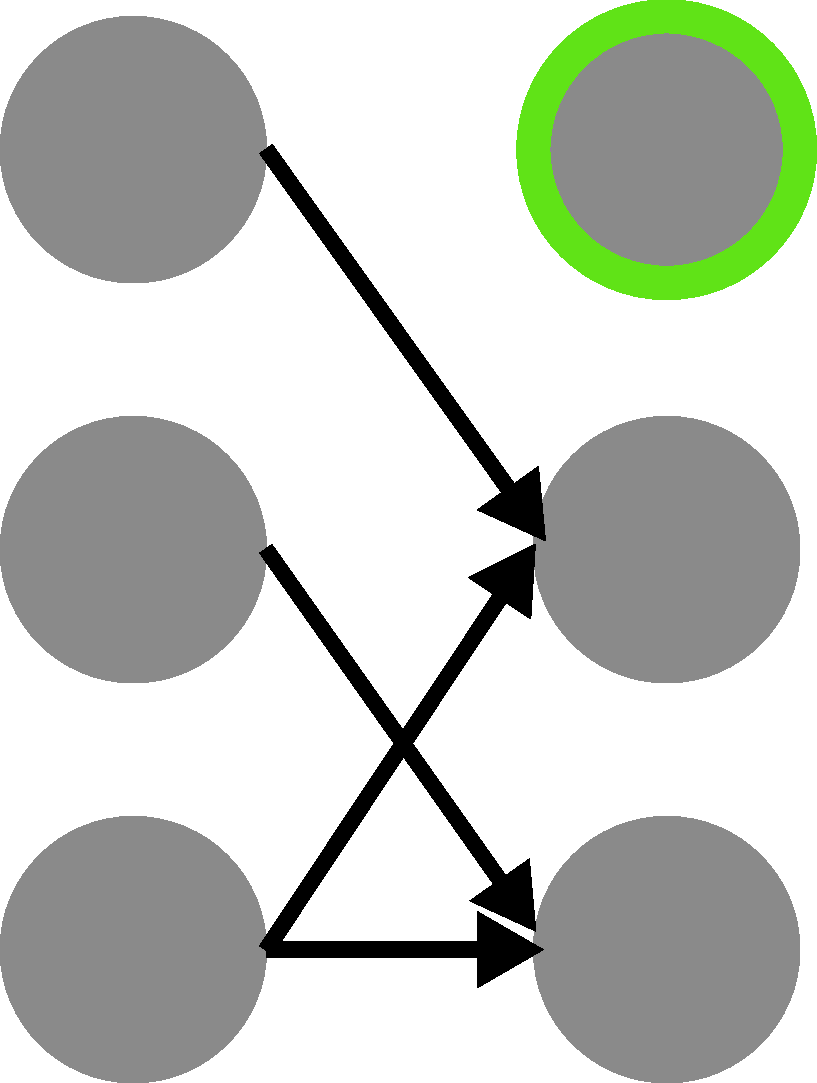
\includegraphics[width = 0.4\textwidth]{./figure/forward_prune}
\end{figure}

\end{block}

\column{.45\textwidth}

\begin{block}{Backward pruning}

$ \forall t \in \{ 1, \cdots T-1 \}, $ \\
$ \forall v \in V(t), deg^{+}(v) > 0 $

\begin{figure}
\centering
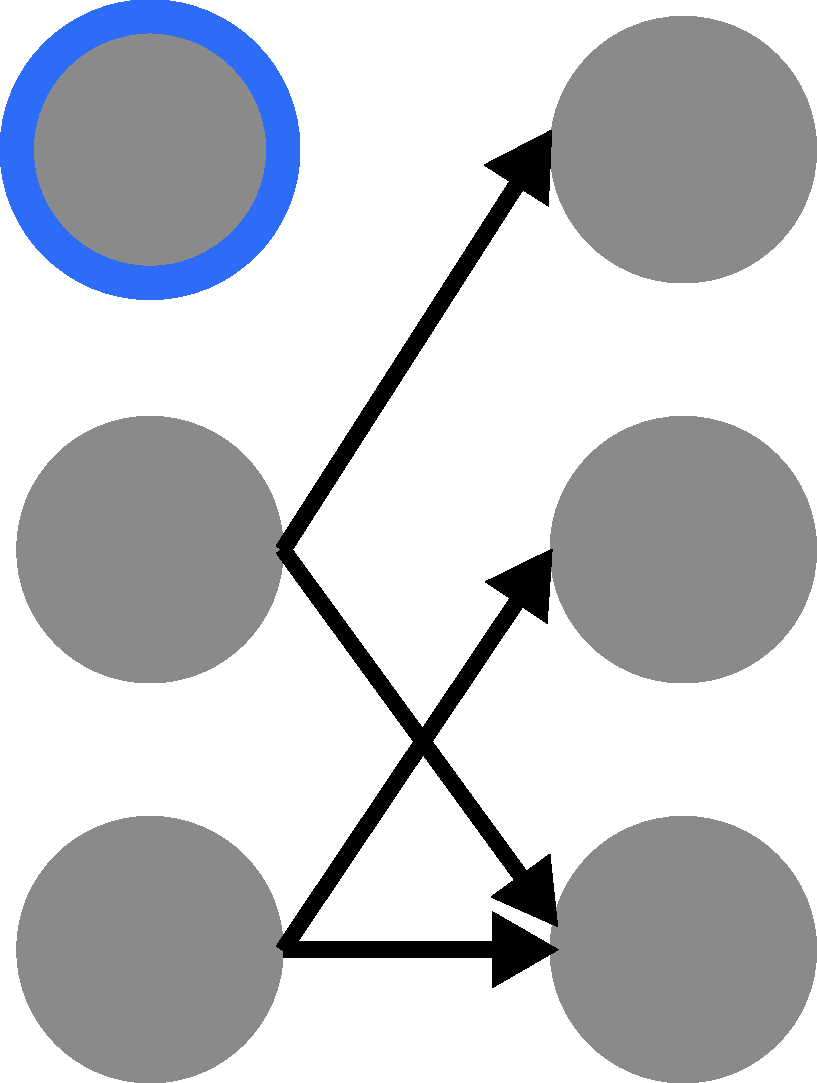
\includegraphics[width = 0.4\textwidth]{./figure/backward_prune}
\end{figure}

\end{block}

\end{columns}

\end{frame}

\begin{frame}{Obstacles}{The optimization model}

\begin{figure}
\centering
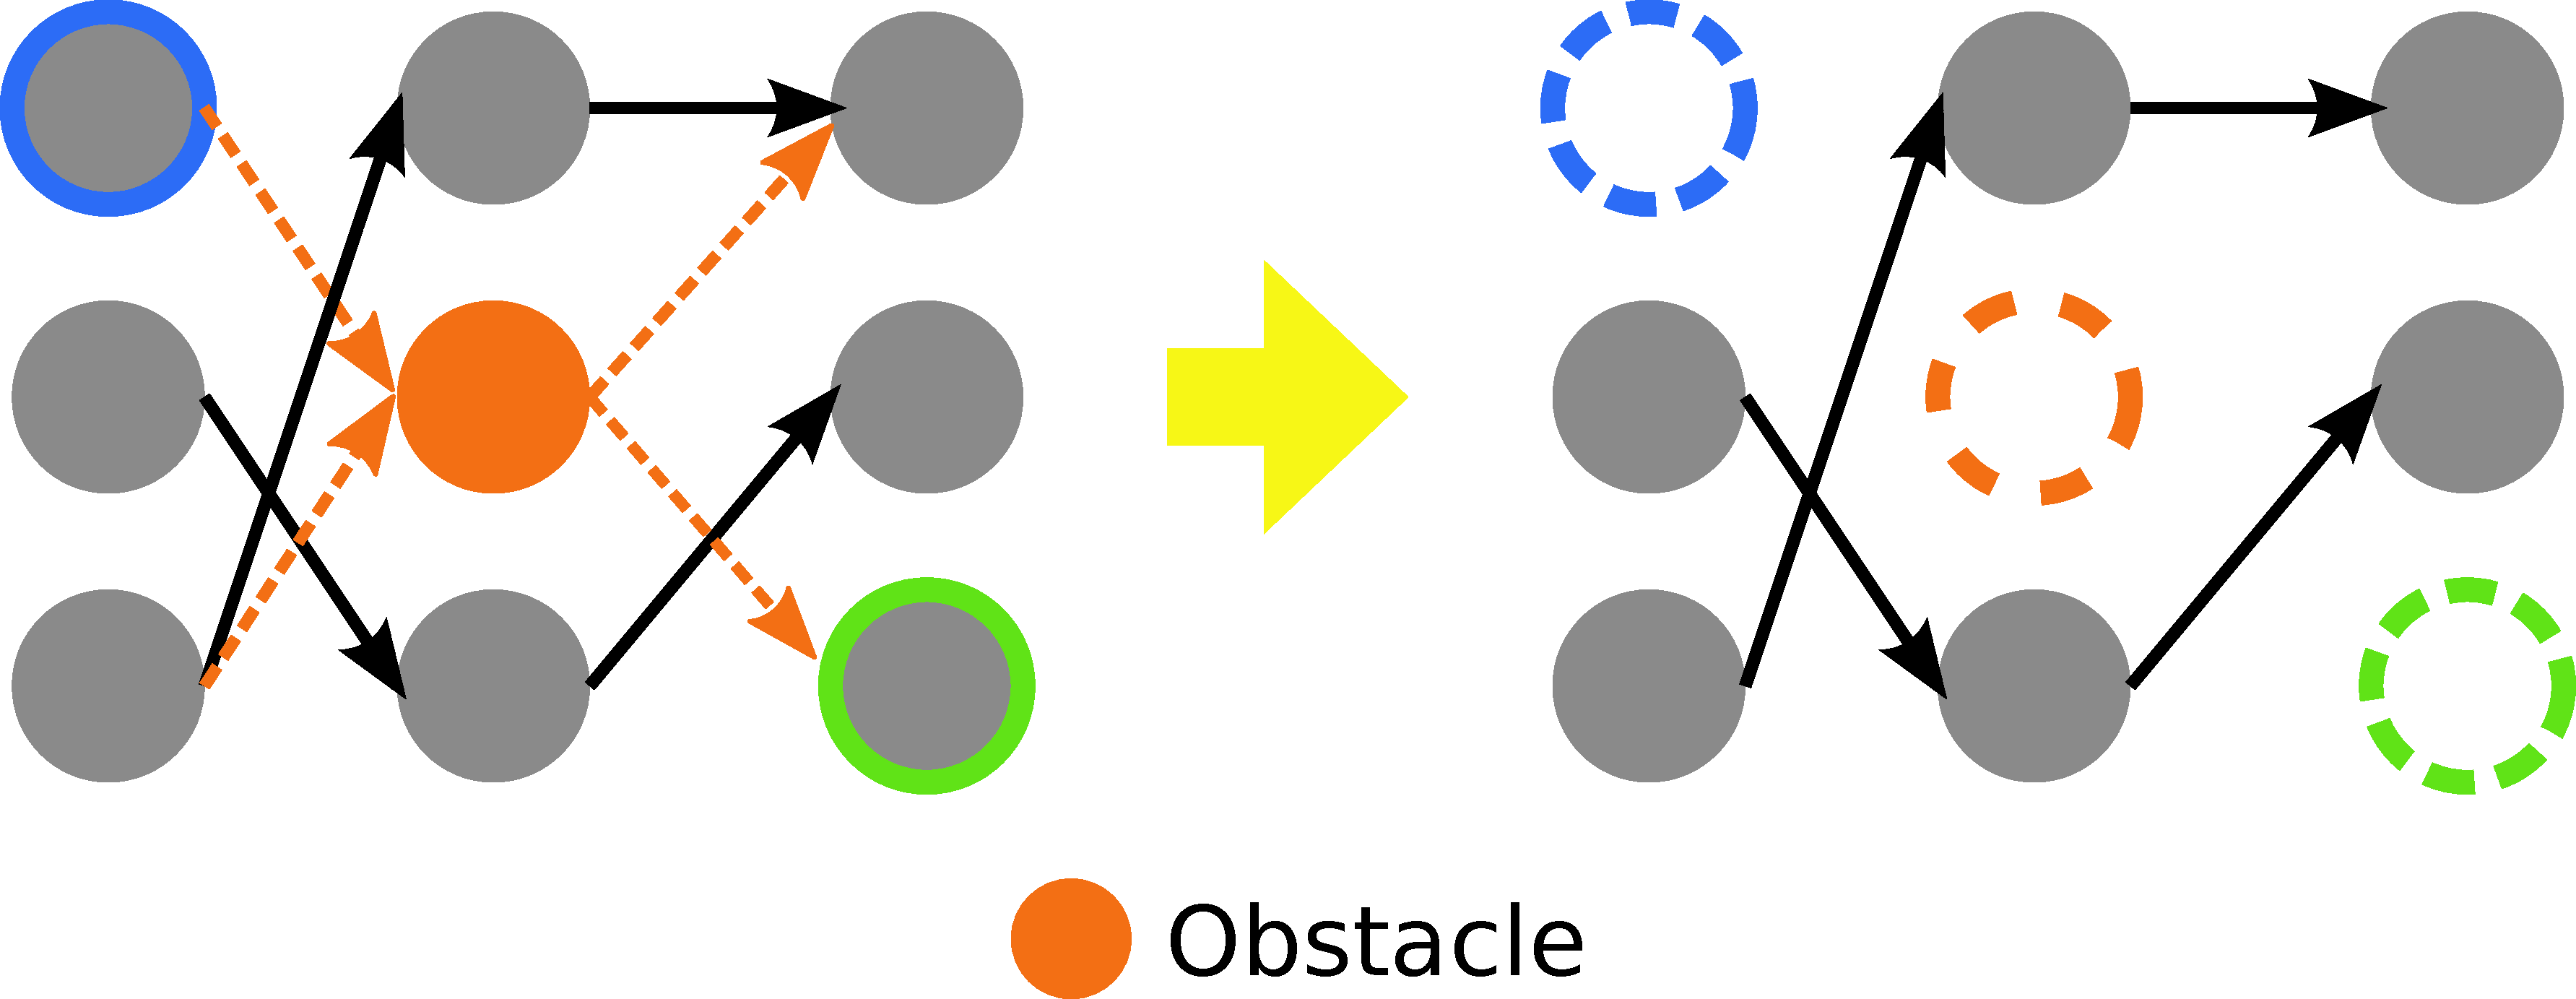
\includegraphics[width = 0.8\textwidth]{./figure/obstacle}
\end{figure}

\end{frame}

\begin{frame}{Submodular orienteering on a multi-partite graph}{The optimization problem}

\begin{equation}
\nonumber
\begin{aligned}
Objective: & X^{*} = \argmax_{X} \: f(X); \\
Constraint: & |X| = T, x_{t} \in V(t), (x_{t}, x_{t+1}) \in E.
\end{aligned}
\end{equation}

\end{frame}



\section{Solution}

\subsection{Backtracking heuristic}

\begin{frame}{Bellman-like equation}{Heuristic}

%\begin{equation}
%\nonumber
%\hat{x}_{t} = \argmax_{X_{t}} [ f(x_{t} \mid x_{1} , \cdots , x_{t-1}) + \max_{X_{t+1}, \cdots , X_{T}} f(x_{t+1}, \cdots , x_{T} \mid x_{1}, \cdots , x_{t}) ]
%\end{equation}

\centering
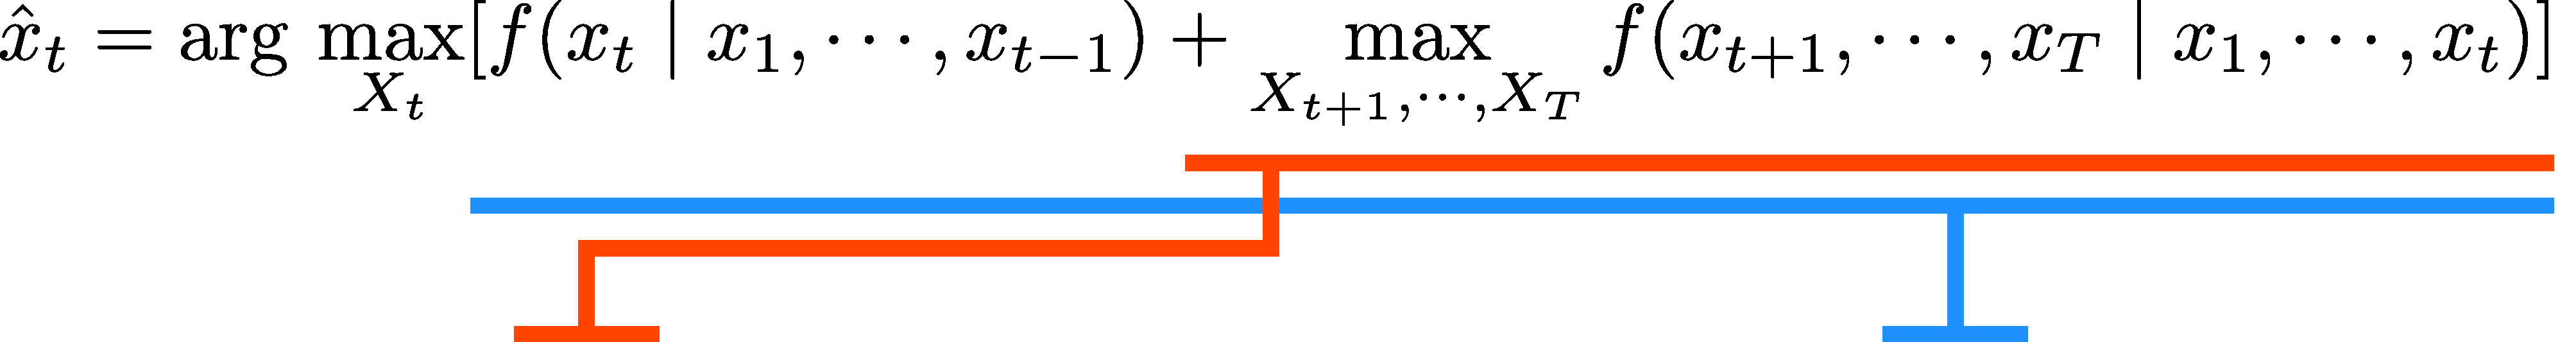
\includegraphics[width = \textwidth]{./figure/arg_equation}

\begin{columns}
\column{0.45\textwidth}
\begin{block}{Maximum future reward}
\begin{figure}
\centering
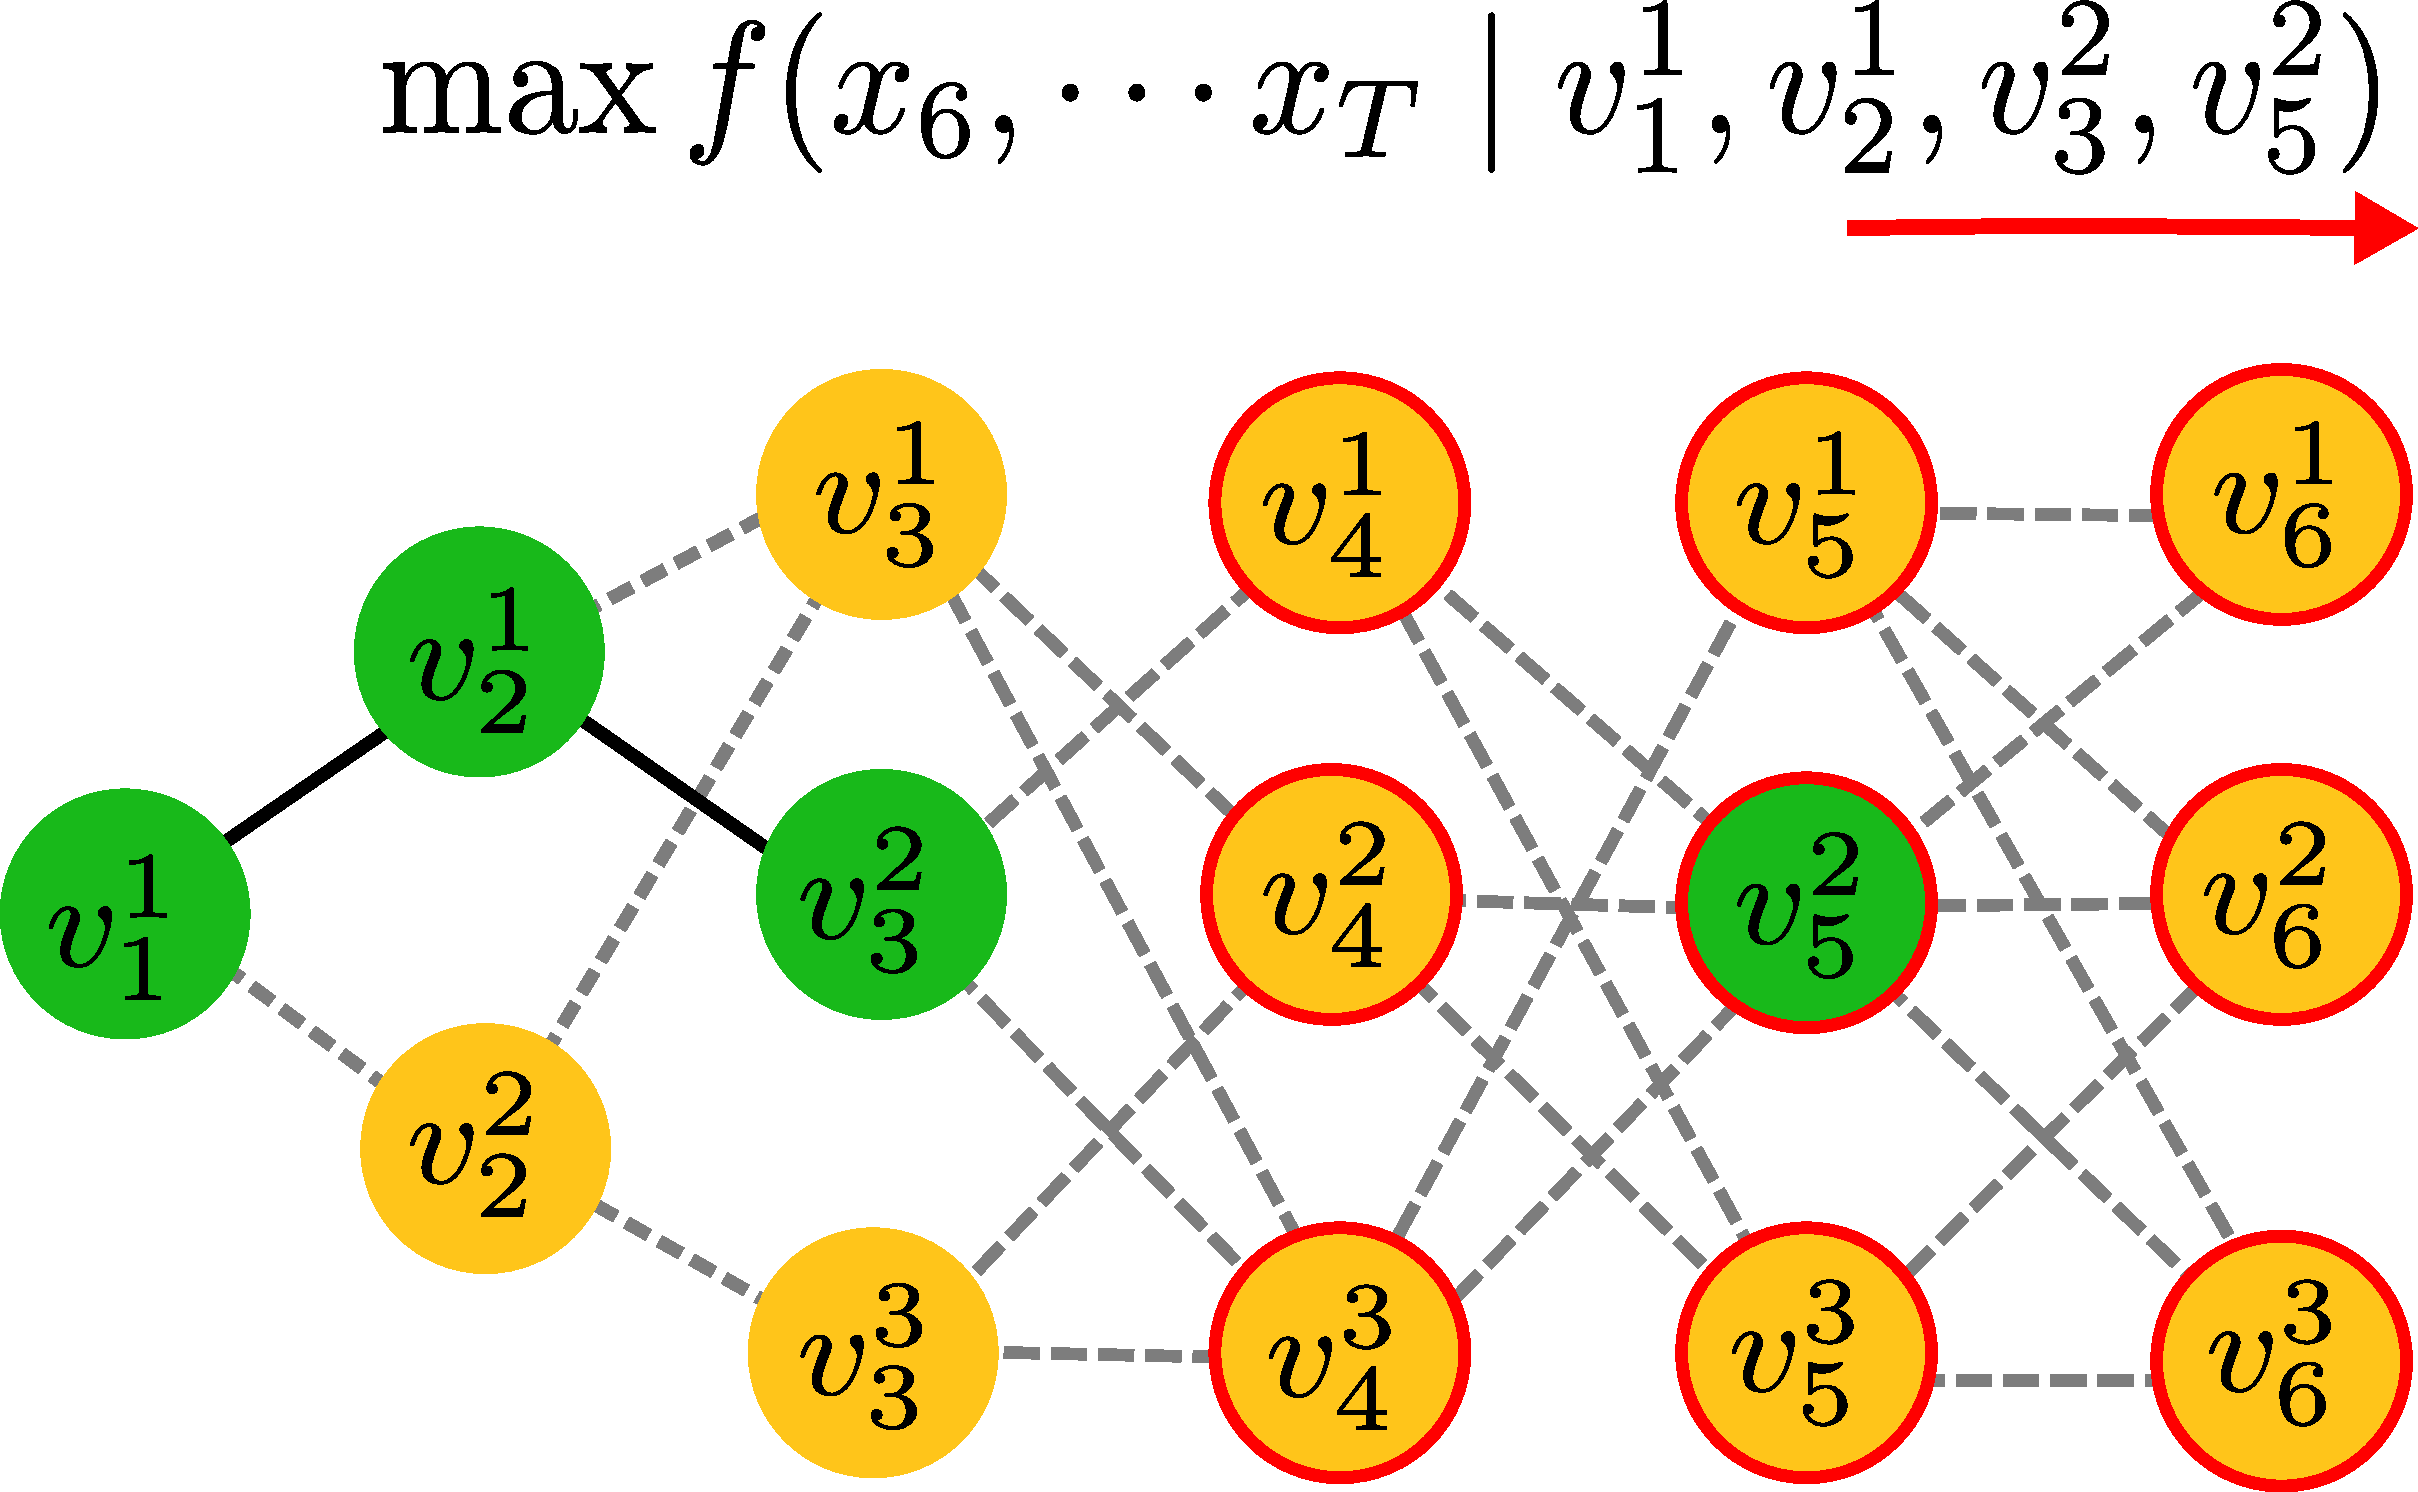
\includegraphics[width = 0.9\textwidth]{./figure/DefineFuncH}
\end{figure}
\end{block}

\column{0.45\textwidth}
\begin{block}{Maximum total reward}
\begin{figure}
\centering
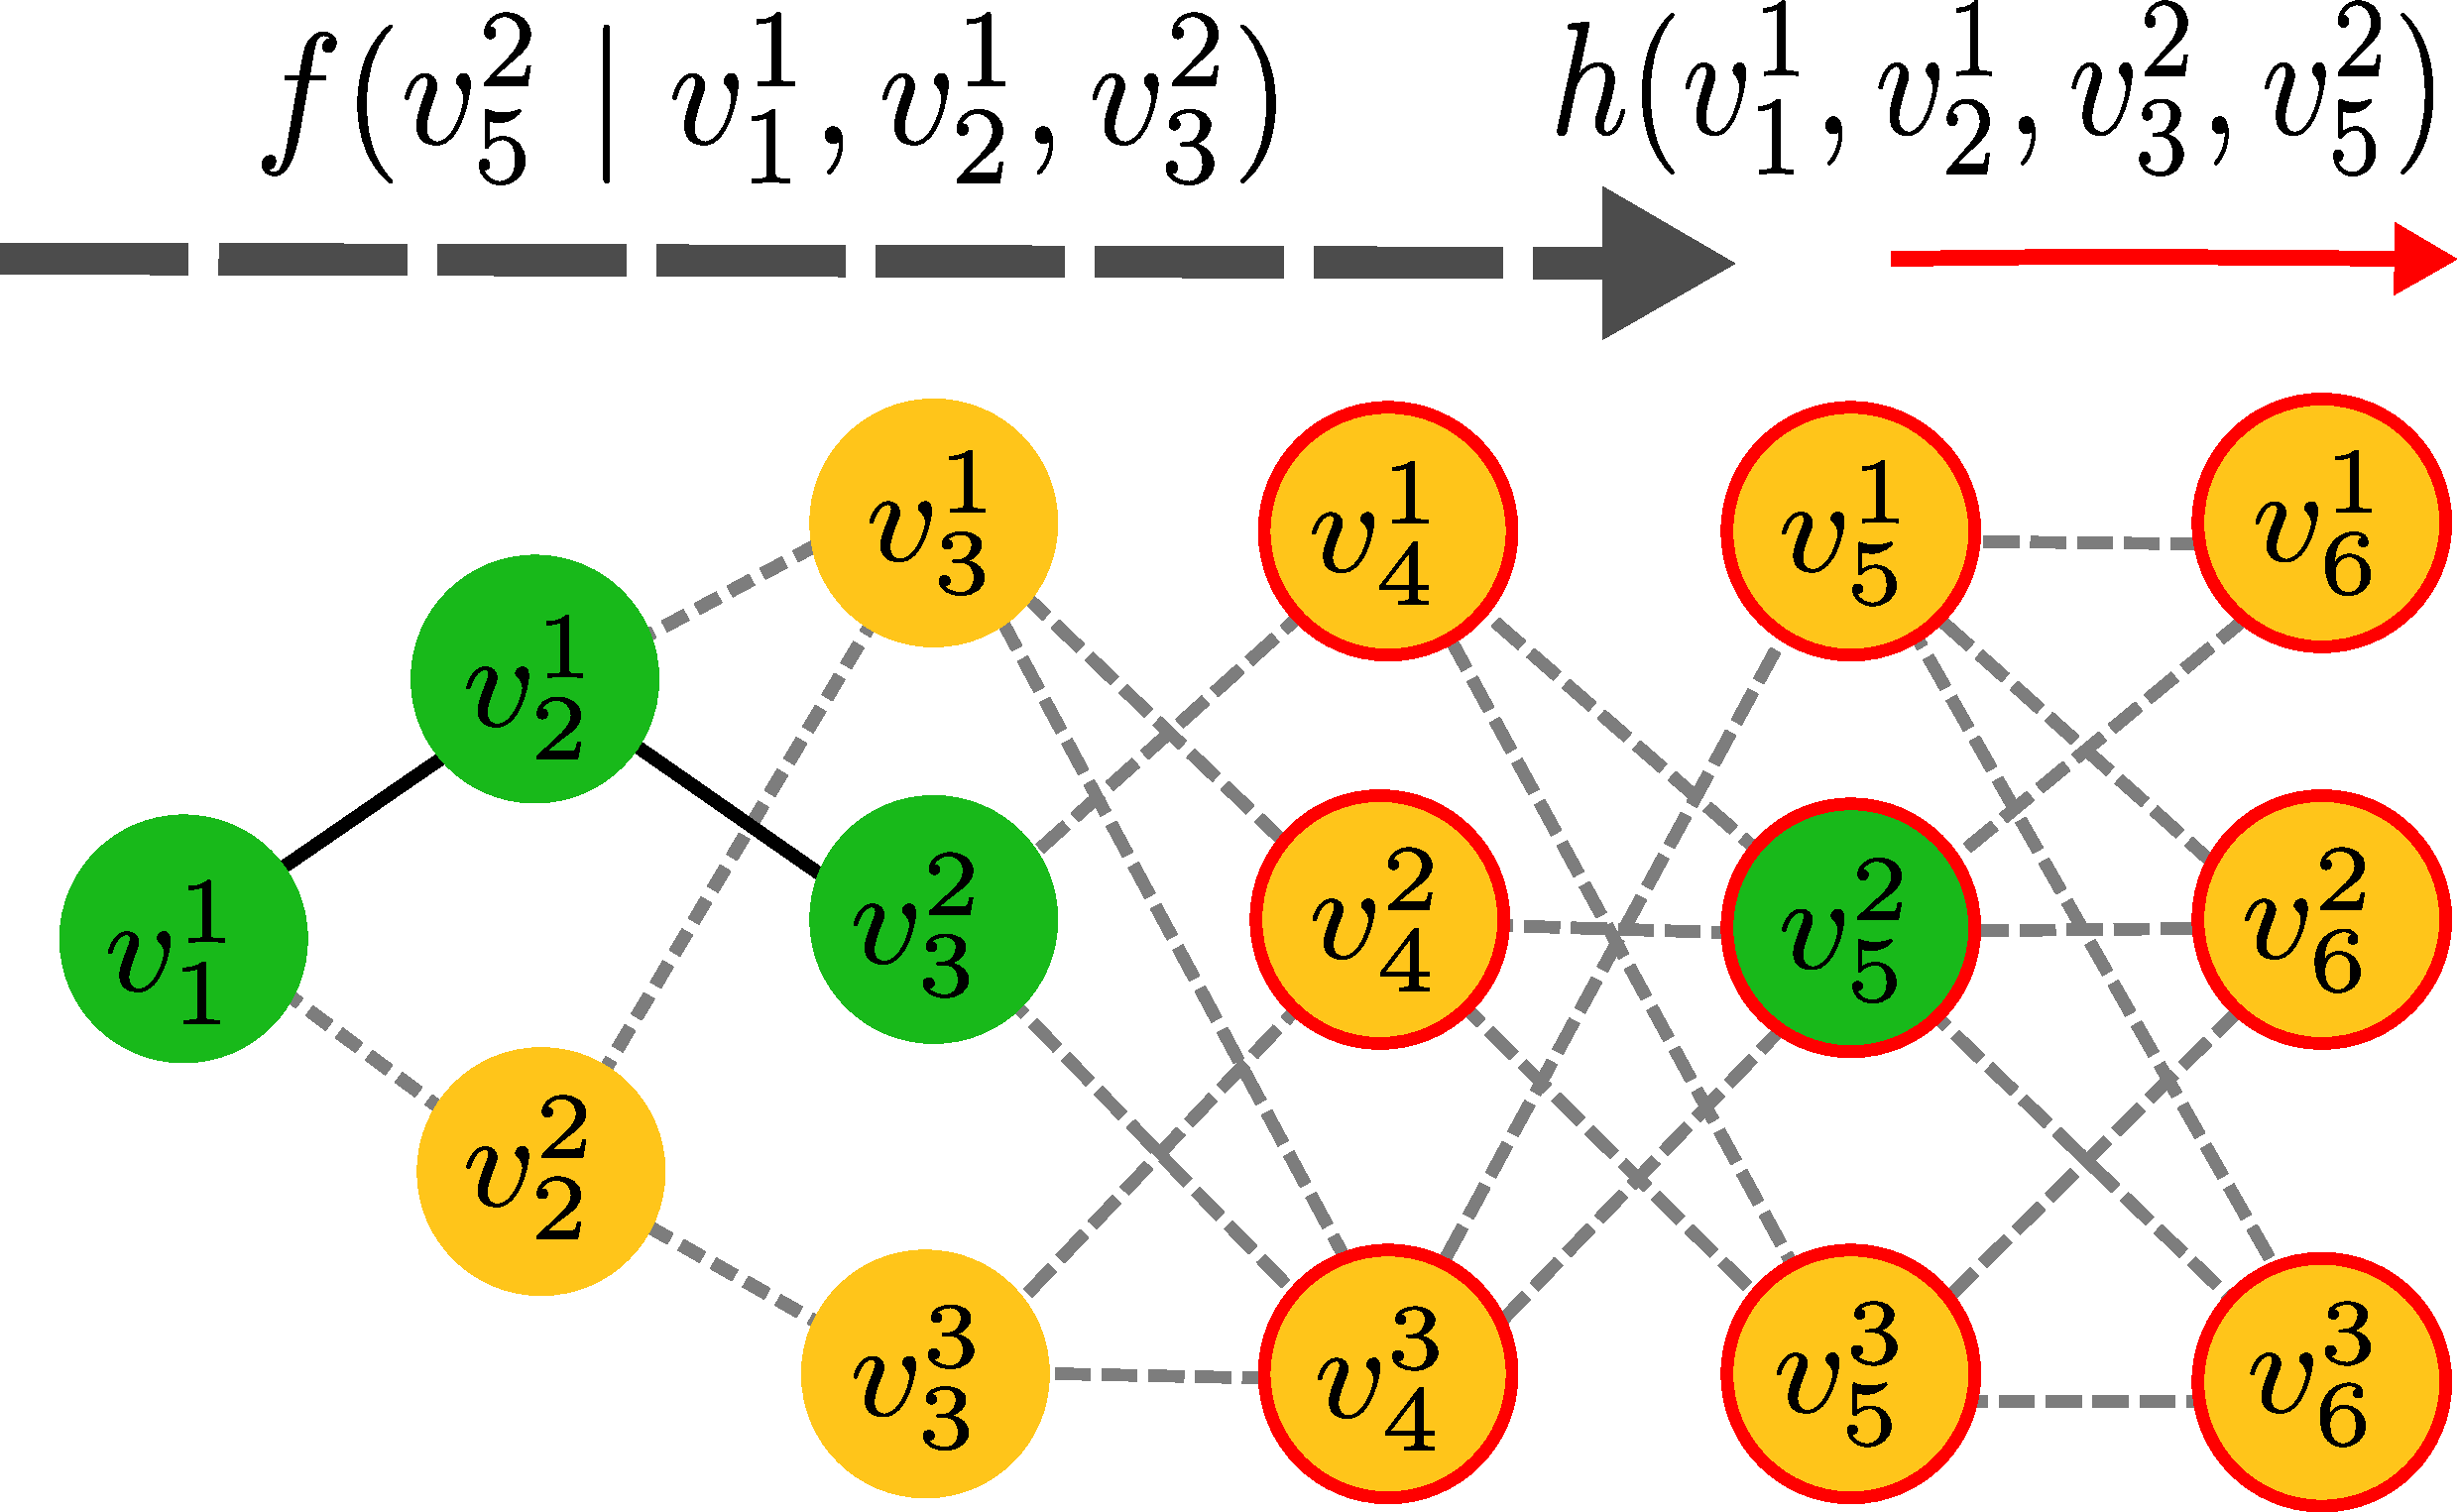
\includegraphics[width = 0.9\textwidth]{./figure/DefineFuncP}
\end{figure}
\end{block}
\end{columns}

\begin{figure}
\centering

\includegraphics[width = 0.9\textwidth]{./figure/DefineFuncHelp}
\end{figure}

\end{frame}

\begin{frame}{Backtracking}{Heuristic}

\begin{columns}

\column{0.6\textwidth}
\begin{minipage}{\textwidth}
\begin{figure}
\centering
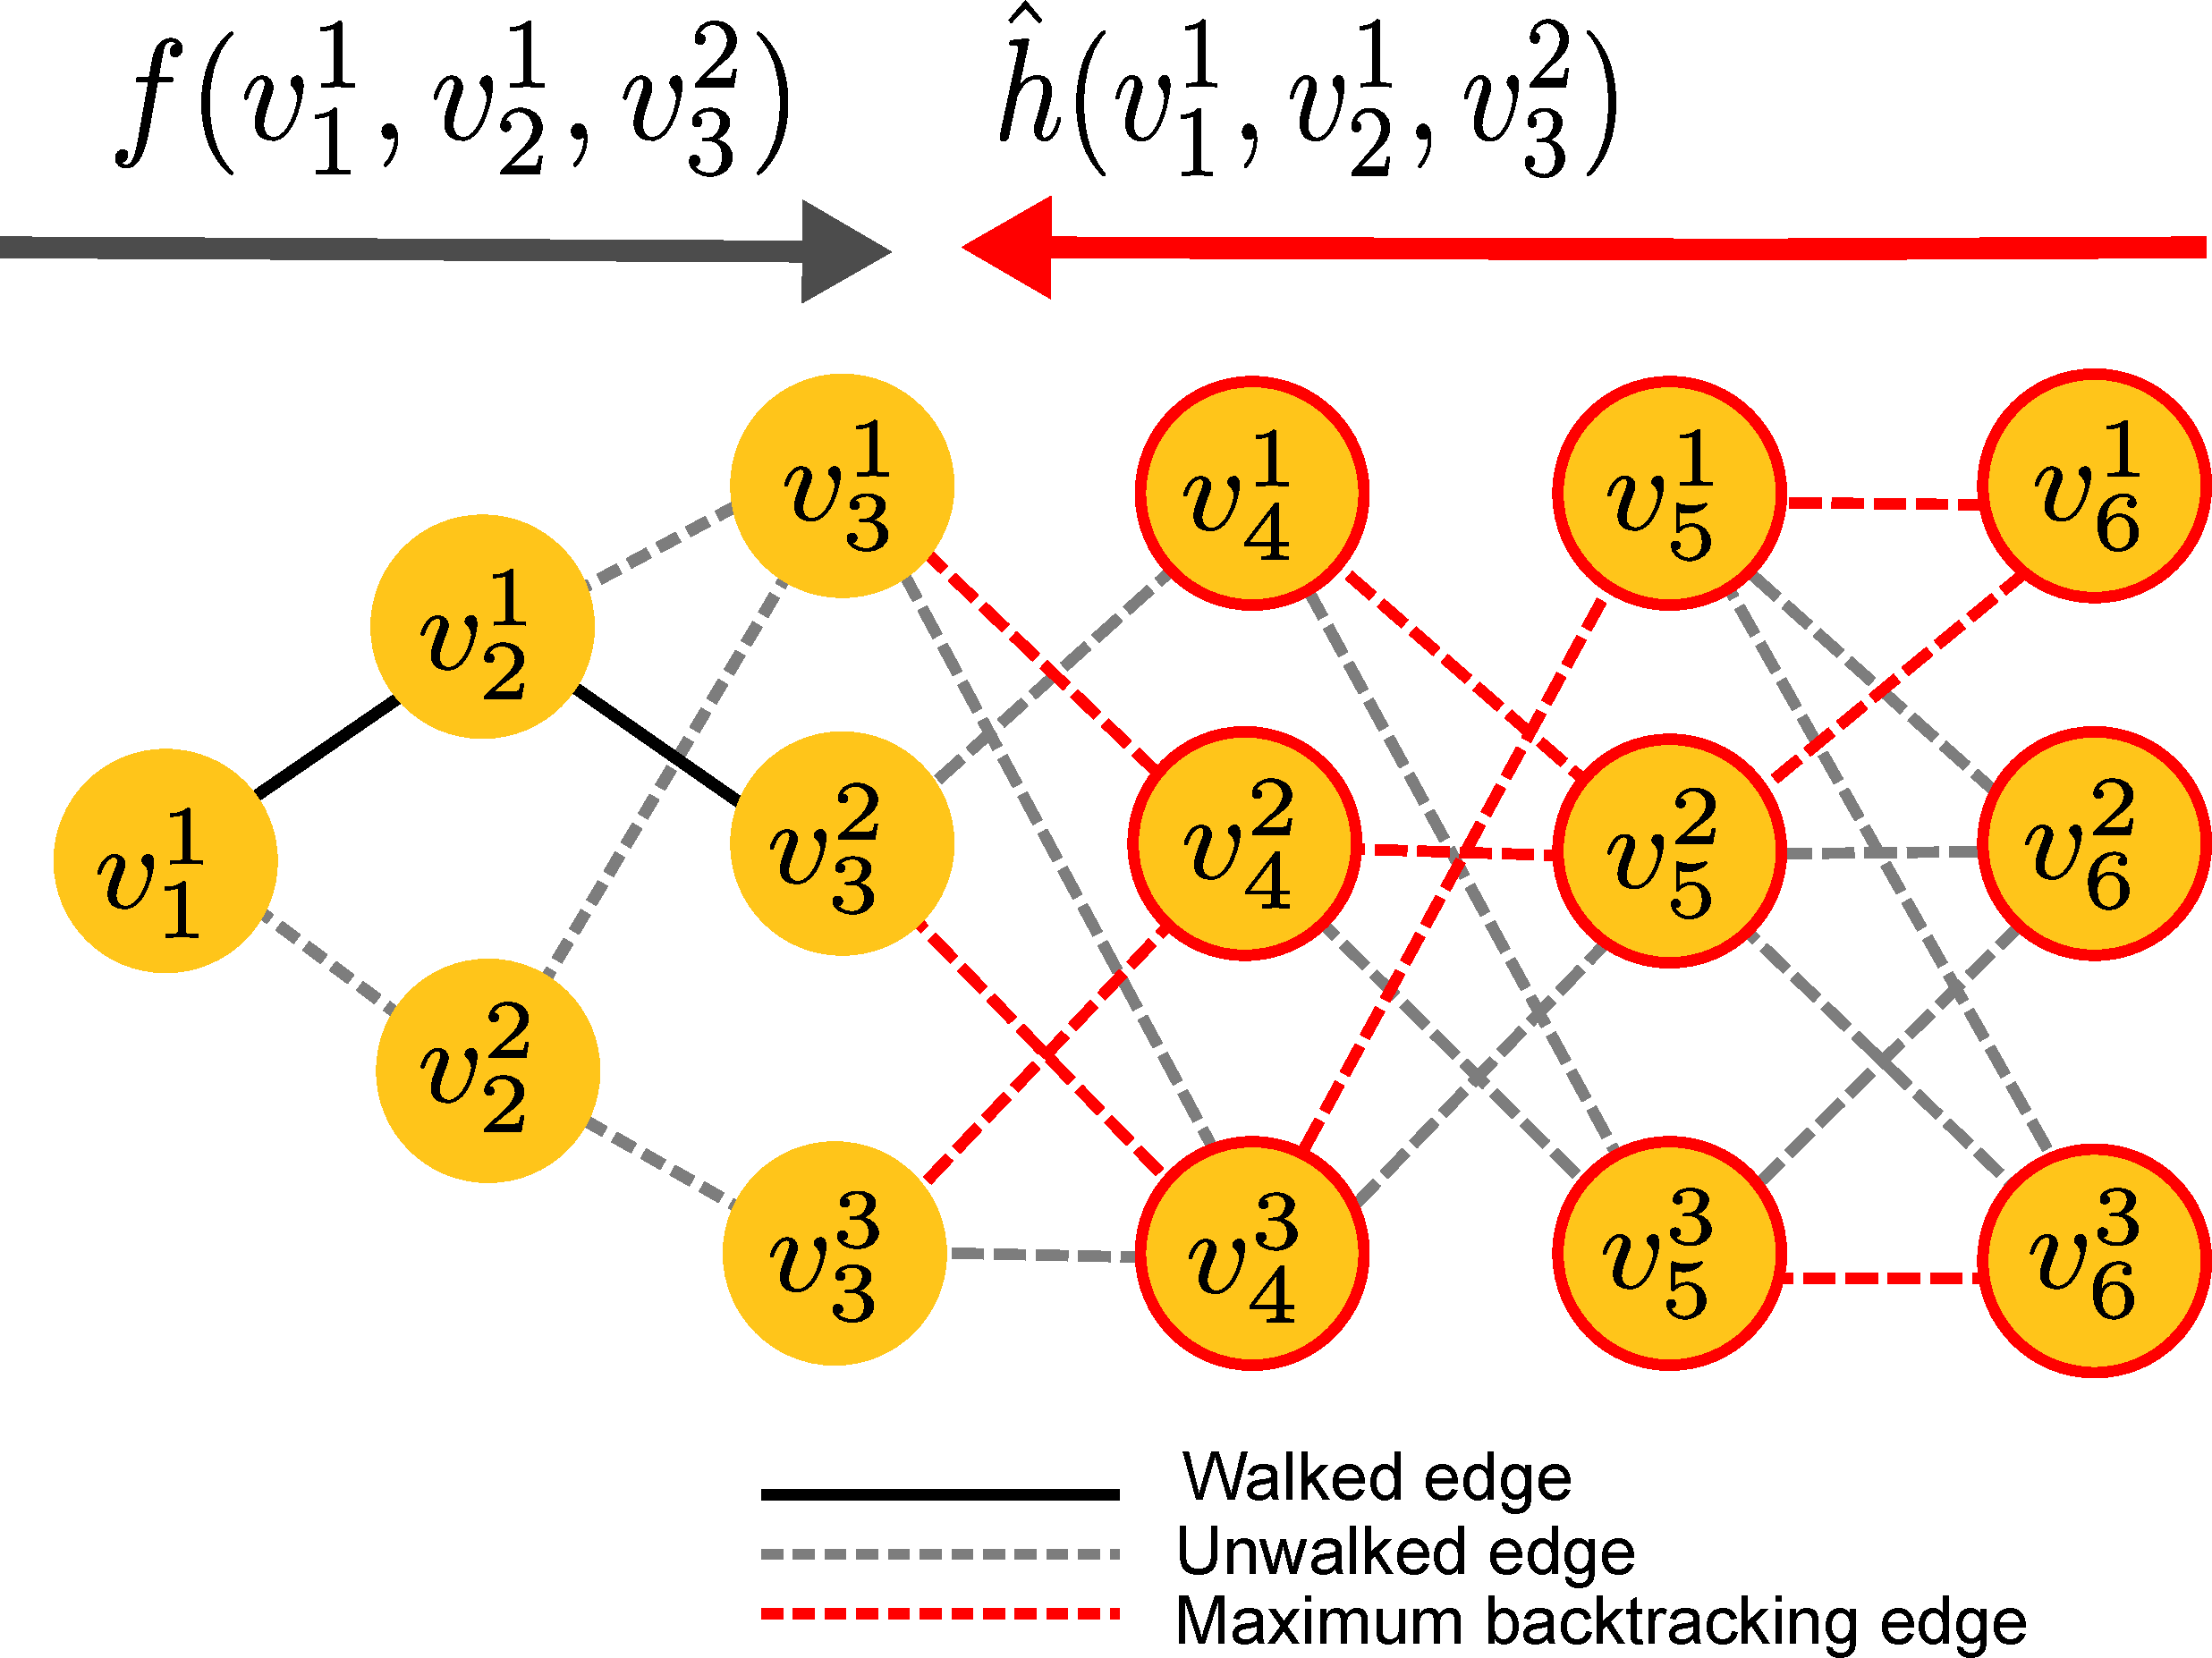
\includegraphics[width = \textwidth]{./figure/backtracking}
\end{figure}
\end{minipage}

\column{0.4\textwidth}
\begin{minipage}{\textwidth}
\begin{itemize}
\item point model $ \rightarrow $ true max total reward
\item coverage model $ \rightarrow $ estimated max total reward guarantee
\end{itemize}
\end{minipage}

\end{columns}

\end{frame}

\subsection{Anytime algorithm design}

\begin{frame}{Expanding tree}{Anytime algorithm framework}

\begin{columns}

\column{0.6\textwidth}
\begin{minipage}{\textwidth}
\begin{figure}
\centering
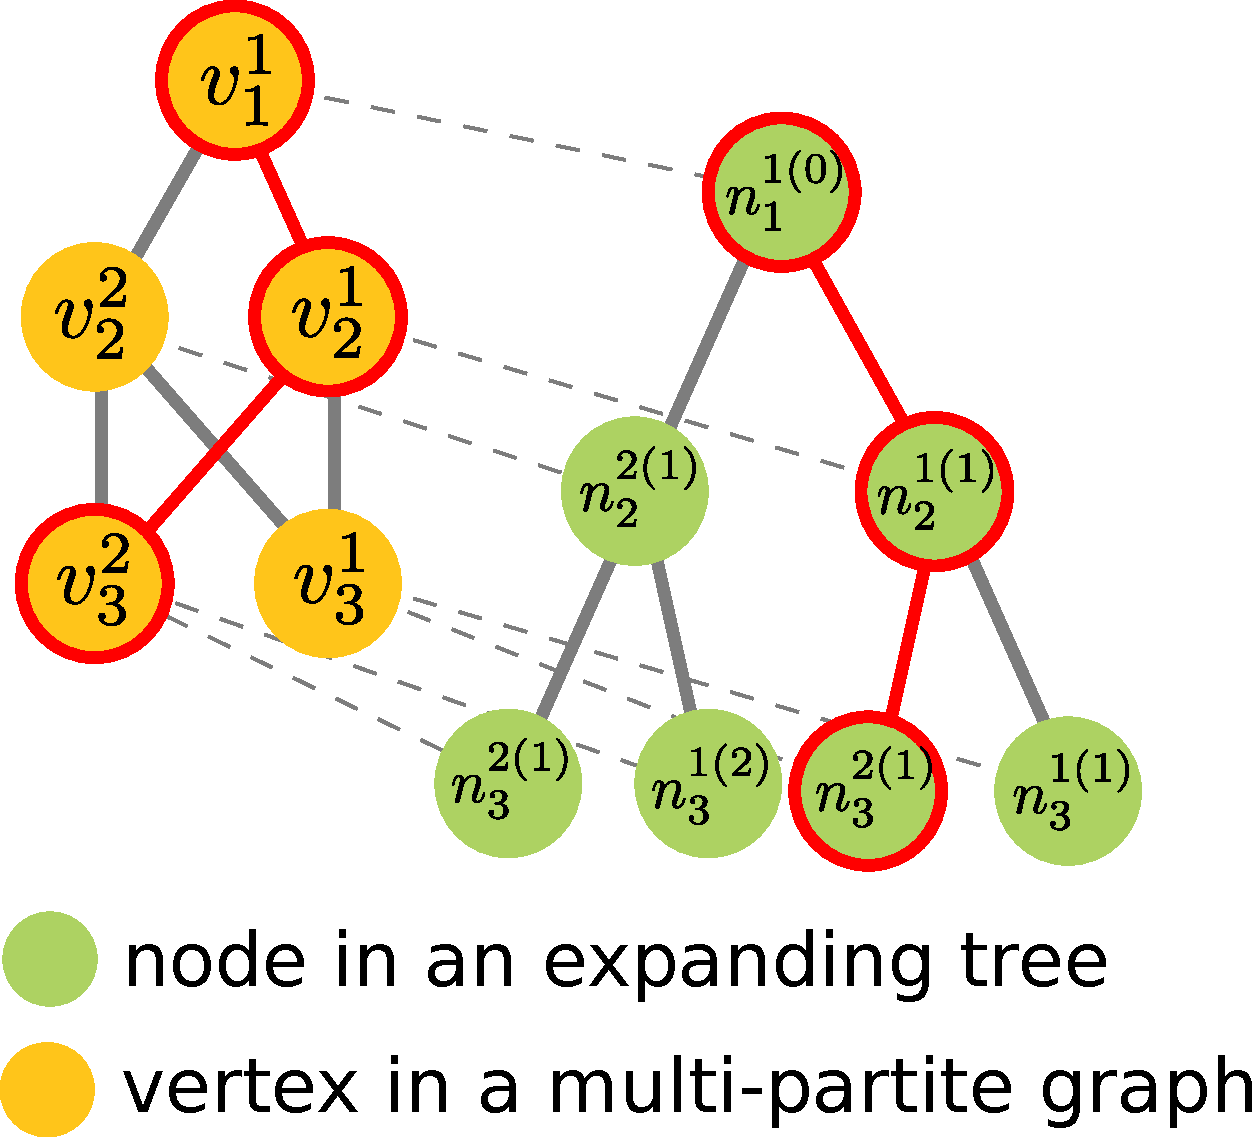
\includegraphics[width=.9\textwidth]{./figure/multipartite_expandingtree}
\end{figure}
\end{minipage}

\column{0.4\textwidth}
\begin{minipage}{\textwidth}
\begin{itemize}
\item depth-first recursive traverse
\item node $ \Longleftrightarrow $ subpath
\item tracking the search process
\item estimation storage
\end{itemize}
%Exapnding tree $ G_{T} = (N, L, T) $ \\
%\begin{itemize}
%\item $ T $ - tree depth
%\item $ N $ - Node set
%\item $ L $ - directed link set
%\end{itemize}
\end{minipage}

\end{columns}

\end{frame}

\begin{frame}{Node freeze}{Anytime algorithm framework}

Estimated reward $ \leq $ Current best reward 
$ \Longrightarrow $ Stop exploring subpath

\begin{figure}
\centering
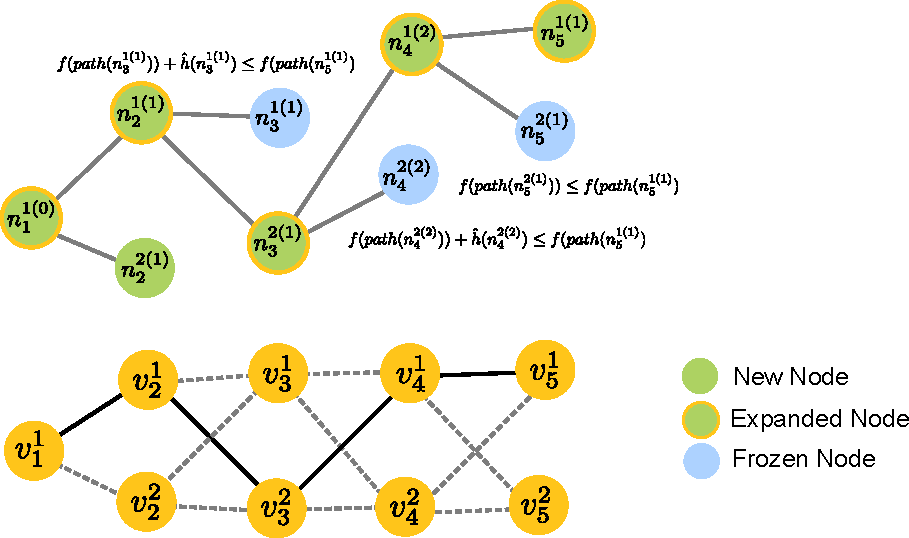
\includegraphics[width =  0.8\textwidth]{./figure/freeze_process}
\end{figure}

\end{frame}

\begin{frame}{Flow}{Anytime algorithm framework}

\begin{figure}
\centering
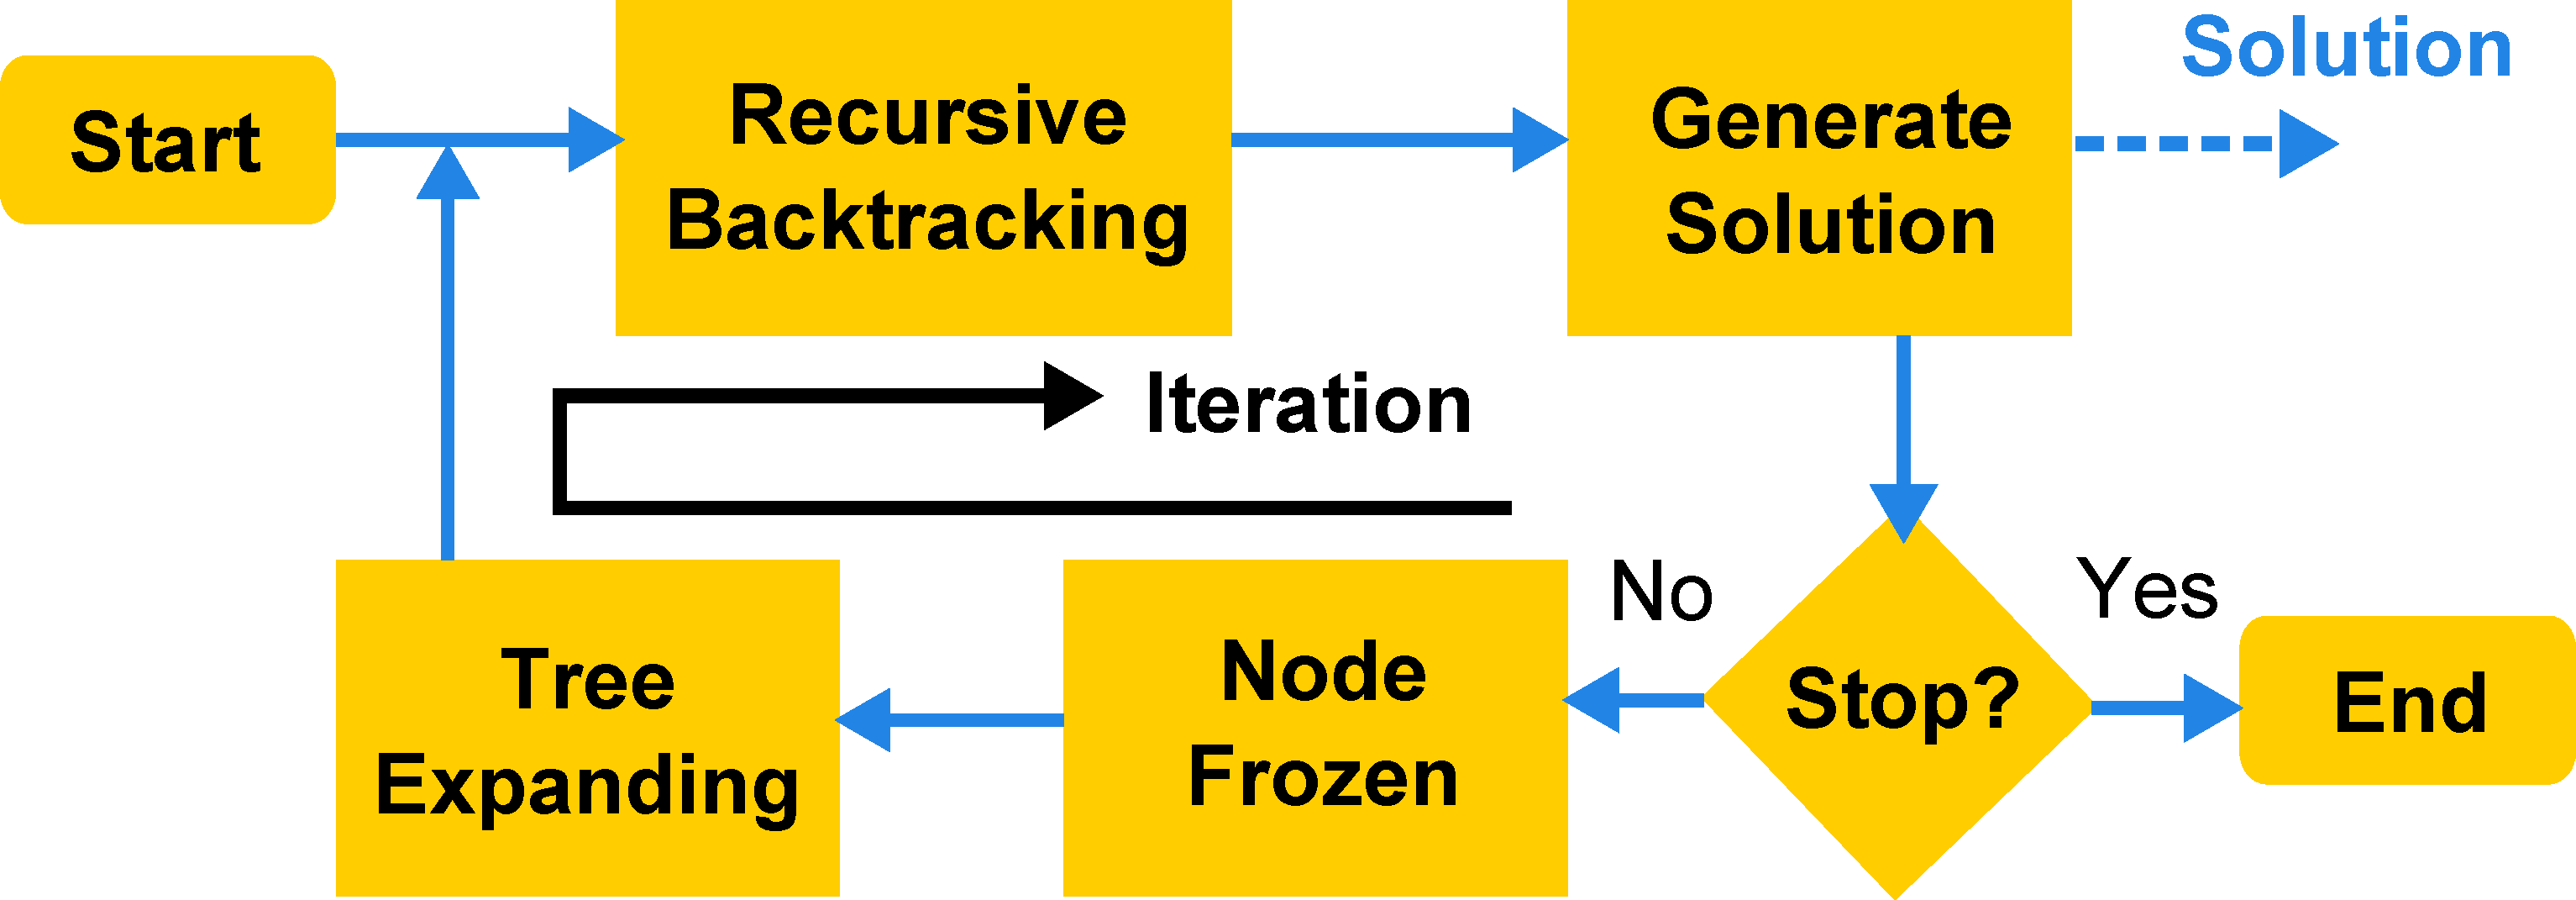
\includegraphics[width = 0.9\textwidth]{./figure/alg_flow}
\end{figure}

\end{frame}

\begin{frame}{Performance guarantee}{Anytime algorithm framework}

\begin{lemma}
“Backtracking” in Algorithm 1 never \textcolor{red}{underestimates}
the maximum total reward, which means
\begin{equation}
\nonumber
\forall t \geq t', \hat{u}(x_{t} \mid v_{1} , \cdots , v_{t'}) \geq u(x_{t} \mid v_{1} , \cdots , v_{t'}).
\end{equation}
\end{lemma}

\begin{minipage}{\textwidth}
\begin{figure}
\centering

\includegraphics[width = 0.15\textwidth]{./figure/arrow}
\end{figure}
\end{minipage}

\begin{theorem}
The anytime algorithm framework in Algorithm 4 can always find an \textcolor{red}{optimal} solution given enough time.
\end{theorem}

\end{frame}






% Placing a * after \section means it will not show in the
% outline or table of contents.
\section{Summary}
\label{sec:summary}

In this paper, we use a human path to form a path constraint and seek to maximize the information gathered by a robot gathered in a search task.
The resulting information maximization path planning is identified as a constrained submodular orienteering problem on a multi-partite graph.
We present an anytime algorithm that used a planning heuristic based on backtracking to efficiently find a high quality path.
We use a node freeze process to avoid an exhaustive search, yet we prove that this process always preserves the ability of the algorithm to find an optimal solution.
We have also shown empirically that this approach substantially reduces the complexity of the resulting search.

% All of the following is optional and typically not needed. 
\section*{Appendix}

\subsection{ISS-Lyapunov function}
\label{sec:iss_lyapunov:func}

Using the definitions of a $ K $-function and a $ KL $-function in Section \ref{sec:system}
we can define a ISS-Lyapunov function as follows,
%\begin{itemize}
%\item 
an ISS-Lyapunov function $ V : \mathbb{R}^{n} \rightarrow \mathbb{R}_{\geq 0} $ satisfies:
\begin{enumerate}
\item $ \exists \alpha_{1}, \alpha_{2} \in \mathbb{K} $ such that 
$ \forall \xi \in \mathbb{R}^{n} $ , $ \alpha_{1} ( | \xi | ) \leq V( \xi ) \leq \alpha_{2}  ( | \xi | ) $.
\item $ \exists \alpha_{3} \in \mathbb{K}_{\infty} , \sigma \in \mathbb{K} $ such that $ \forall \xi \in \mathbb{R}^{n}, \forall \mu \in \mathbb{R}^{m} $,$  V( f( \xi, \mu ) ) - V( \xi ) \leq - \alpha_{3} ( | \xi | ) + \sigma ( | \mu | ) $. 
\end{enumerate}

\subsection{Proof of Theorem \ref{thm:iss}}
\label{sec:thm:iss:proof}
		
\begin{proof} 
Let $ P $ be an identity matrix.
As $ | \lambda_{\max} ( A(k) ) | < 1 $, we have
%\begin{equation}
%\nonumber
$
\lVert A^{T}(k) P A(k) \rVert \leq \lVert P \rVert \lVert A(k) \rVert^{2} \leq \lVert P \rVert | \lambda_{\max} ( A(k) ) |^{2} $ $  <  \lVert P \rVert .
$
%\end{equation}
Because $ P $ is an identity matrix it is positive definite, and thus $ A^{T}(k) P A(k) $ is positive definite or positive semi-definite by definition.
So by positive definite ordering we have $ A^{T}(k) P A(k) < P $.
		
Let $ -Q(k) = A^{T}(k) P A(k) - P $. Since $ A^{T}(k) P A(k) < P $ then $ - Q(k) < 0 $ furthermore $ \exists Q' \forall k, Q(k) > Q' > 0 $. 
		
By the Lemma 3.5 in \cite{Jiang2001857}, if we can show that a proposed positive definite Lyapunov function is an ISS-Lyapunov function, then the system is ISS.
		
Define a Lyapunov function
\begin{equation}
\label{eq:lyapunov_v}
V( X(k) ) = X^{T} (k) P X(k).
\end{equation}
We can have
$
\lambda_{min}(P) | X(k) |^{2} \leq V( X(k) )\leq \lambda_{max}(P) | X(k) |^{2}
$ and $ \lambda_{min}(P) = \lambda_{max}(P) $.
		
Let $ \alpha_{1} ( \xi )= \lambda_{min} \xi^{2} $
and 
$ \alpha_{2} ( \xi )= \lambda_{max} \xi^{2} $,
we have $ V(x) $ satisfying condition 1 of the ISS-Lyapunov function definition.
		
By applying equation \eqref{eq:pso_up_linalg_simp} to $ V( X(k+1) ) - V( X(k) ) $, we have
\begin{equation}
\label{eq:lyapunov_delta2}
\begin{aligned}
& V( X(k+1) ) - V( X(k) ) \\
%	= & - X^{T}(k) [ A^{T}(k) P A(k) - P ] X(k) + 2 X^{T}(k)  A^{T}(k) P B(k) U(k) \\
%	& + U^{T}(k) B^{T}(k) P B(k) U(k) \\
%	\leq & - X^{T}(k) Q' X(k) + 2 X^{T}(k)  A^{T}(k) P B(k) U(k) \\
%	& + U^{T}(k) B^{T}(k) P B(k) U(k) \\
%	\leq & - \lambda_{min}(Q') | X(k) |^{2} + 2  \lVert A^{T}(k) P B(k) \rVert  U(k) | | X(k) | \\
%	& + \lVert B^{T}(k) P B(k) \rVert | U(k) |^{2}.
= & [ X^{T}(k)  A^{T}(k) + U^{T}(k) B^{T}(k) ] P [ A(k) X(k) + B(k) U(k) ] \\ & - X^{T}(k) P X(k) \\
= & X^{T}(k)  A^{T}(k) P A(k) X(k) +  X^{T}(k)  A^{T}(k) P B(k) U(k) \\
& + U^{T}(k) B^{T}(k) P A(k) X(k) + U^{T}(k) B^{T}(k) P B(k) U(k) \\ & - X^{T}(k) P X(k) \\
\end{aligned}
\end{equation}
As $ P $ is identity matrix, it is symmetric, thus
\begin{equation}
[ X^{T}(k)  A^{T}(k) P B(k) U(k) ]^{T} =  U^{T}(k) B^{T}(k) P A(k) X(k).
\end{equation}
$ V( X(k+1) ) , V( X(k) ) \in \mathbb{R} $, 
we have $ X^{T}(k)  A^{T}(k) P B(k) U(k) $ and $  U^{T}(k) B^{T}(k) P A(k) X(k) $ are both real value (like $ 1 \times 1 $ matrix).
Thus, 
\begin{equation}
 X^{T}(k)  A^{T}(k) P B(k) U(k) =   U^{T}(k) B^{T}(k) P A(k) X(k) .
\end{equation}
We then have
\begin{equation}
\label{eq:lyapunov_delta3}
\begin{aligned}
& V( X(k+1) ) - V( X(k) ) \\
= & - X^{T}(k) [ A^{T}(k) P A(k) - P ] X(k) \\
& + U^{T}(k) B^{T}(k) P B(k) U(k)  \\
& + 2 X^{T}(k)  A^{T}(k) P B(k) U(k) \\
\leq & - X^{T}(k) Q' X(k)  + U^{T}(k) B^{T}(k) P B(k) U(k) \\
& + 2 X^{T}(k)  A^{T}(k) P B(k) U(k) \\
\end{aligned}
\end{equation}

By applying matrix norm, we have
\begin{equation}
\begin{aligned}
& V( X(k+1) ) - V( X(k) ) \\
\leq & - \lambda_{min}(Q') | X(k) |^{2}  + | B^{T}(k) P B(k) | | U(k) |^{2} \\
& + 2  | A^{T}(k) P B(k) | | U(k) | | X(k) | \\
= & - \frac{1}{2} \lambda_{min}(Q') | X(k) |^{2} + | B^{T}(k) P B(k) | | U(k) |^{2} \\
& - \frac{1}{2} \lambda_{min}(Q') | X(k) |^{2} + 2  | A^{T}(k) P B(k) | | U(k) | | X(k) |  \\
= & - \frac{1}{2} \lambda_{min}(Q') | X(k) |^{2} \\
& + \left( \frac{2 | A^{T}(k) P B(k) |^{2}}{ ( \lambda_{min}(Q') )^{2} } + | B^{T}(k) P B(k) |  \right) | U(k) |^{2} \\
& - \frac{1}{2} \lambda_{min}(Q') [ | X(k) |^{2} - \frac{4 | A^{T}(k) P B(k) | }{ \lambda_{min}(Q') }  | X(k) | | U(k) | \\
& + \frac{4 | A^{T}(k) P B(k) |^{2}}{ ( \lambda_{min}(Q') )^{2} } | U(k) |^{2} ] \\
\end{aligned}
\end{equation}
		
By completing the square, we have
\begin{equation}
\label{eq:lyapunov_delta4}
\begin{aligned}
& V( X(k+1) ) - V( X(k) ) \\
= & - \frac{1}{2} \lambda_{min}(Q') | X(k) |^{2} \\
& + \left( \frac{2 | A^{T}(k) P B(k) |^{2}}{ ( \lambda_{min}(Q') )^{2} } + | B^{T}(k) P B(k) | \right) | U(k) |^{2} \\
& - \frac{1}{2} \lambda_{min}(Q') \left( | X(k) | - \frac{2 | A^{T}(k) P B(k) | }{ \lambda_{min}(Q') } | U(k) | \right)^{2} \\
	\leq & - \frac{1}{2} \lambda_{min}(Q') | X(k) |^{2} \\
 &	+ \left( \frac{2 \lVert A^{T}(k) P B(k) \rVert^{2}}{ ( \lambda_{min}(Q') )^{2} } 
	 + \lVert B^{T}(k) P B(k) \rVert \right) | U(k) |^{2}. 
\end{aligned}
\end{equation}
		
Because $ u^{P}(k) \in [0, 1] $, there exist an $ A' $ and $ B' $ such that $ \lVert A(k) \rVert \leq \lVert A' \rVert $ and $ \lVert B(k) \rVert \leq \lVert B' \rVert $.
We have $ \lVert A^{T}(k) P B(k) \rVert $ $  \leq \lVert A' \rVert \lVert P \rVert \lVert B' \rVert $ and $ \lVert B^{T}(k) P B(k) \rVert \leq \lVert P \rVert \lVert B' \rVert^{2} $.
		
Since the identity matrix $ P $ has $ || P || = 1 $:
\begin{equation}
\label{eq:lyapunov_delta5}
\begin{aligned}
& V( X(k+1) ) - V( X(k) ) \\
	\leq & - \frac{1}{2} \lambda_{min}(Q') | X(k) |^{2} + \left( \frac{2 \lVert A' \rVert^{2} \lVert B' \rVert^{2}}{ ( \lambda_{min}(Q') )^{2} } + \lVert B' \rVert^{2} \right) | U(k) |^{2}.
\end{aligned}
\end{equation}
		
Let
\begin{equation}
\nonumber
\alpha_{3} ( \xi )= \frac{1}{2} \lambda_{min}(Q') \xi^{2} ,
\end{equation}
and
\begin{equation}
\nonumber
\sigma ( \xi ) = \left( \frac{2 \lVert A' \rVert^{2} \lVert B' \rVert^{2}}{ ( \lambda_{min}(Q') )^{2} } +  \lVert B' \rVert^{2} \right) \xi^{2} .
\end{equation} 
Thus we have $  V( X(k+1) ) - V( X(k) ) $ satisfying condition 2 of the ISS-Lyapunov function definition and
so \eqref{eq:lyapunov_v} is an ISS-Lyapunov function.
Using Jiang's Lemma 3.5\cite{Jiang2001857}, the position-update component of PSO (equation \eqref{eq:pso_up_linalg_simp}) is input-to-state stable.
\end{proof}

\subsection{Proof of Corollary \ref{coro:param_unit_disc}}
\label{sec:coro:param_unit_disc:proof}

\begin{proof}
Let $ a = (1 + \chi) - \chi \phi $. 
The eigenvalues of $ A(k) $ are
\begin{equation}
\nonumber
 \lambda = \frac{ a \pm \sqrt{ a^{2} - 4 \chi } }{2} .
\end{equation}
There can be two cases.		
\begin{enumerate}
\item If $ a^{2} \geq 4 \chi $, the eigenvalues are complex number.
We have $ a \geq 2 \sqrt{\chi} $ or $ a \leq - 2 \sqrt{\chi} $.
			
If $ a \geq 2 \sqrt{\chi} $, then $ | \lambda_{\max} | < 1 $ derives 
\begin{equation}
\nonumber
0 < \frac{a-\sqrt{a^{2}-4\chi}}{2} \leq \frac{a+\sqrt{a^{2}-4\chi}}{2} < 1 .
\end{equation}
It means that $ 2 \sqrt{ \chi } \leq a < 1 + \chi $.
			
If $ a \leq 2 \sqrt{\chi} $, then $ | \lambda_{\max} | < 1 $ derives
\begin{equation}
\nonumber
-1 < \frac{a-\sqrt{a^{2}-4\chi}}{2} \leq \frac{a+\sqrt{a^{2}-4\chi}}{2} < 0 .
\end{equation}
It means that $ - (\chi+1) < a \leq - 2 \sqrt{\chi} $.
			
\item If $ a^{2} < 4 \chi $, the eigenvalues are real number.
We have $ - 2 \sqrt{\chi} < a < 2 \sqrt{\chi} $.
			
$ | \lambda_{\max} | < 1 $ derives
\begin{equation}
\nonumber
\frac{ a^{2} }{4} + \frac{ a^{2} - 4\chi }{4} < 1 .
\end{equation}
It means that $ - 2 \sqrt{ 2(1+\chi) } < a < 2 \sqrt{ 2(1+\chi) } $.
Because $ \sqrt{ 2(1+\chi) } > 2 \sqrt{ \chi } $, we have $ - 2 \sqrt{\chi} < a < 2 \sqrt{\chi} $.
\end{enumerate}
Combining these two cases, we have  $ - (1 + \chi) < a < 1 + \chi $.
It equals to $ \phi \in \left( 0 , \frac{2(1+\chi)}{\chi} \right) $.
\end{proof}	

\subsection{Proof of the Theorem \ref{thm:state_bound}}	
\label{sec:thm:state_bound:proof}

\begin{proof}
As we have the update equation as
$ X(k+1) = A(k) X(k) + B(k) U(k) $, we can derive 
\begin{equation}
X(k+1) = ( \prod_{k}^{i=0} A(i) ) X(0) + \sum_{i=0}^{k} [ ( \prod_{j=0}^{i-1} A(j) ) B(i) U(i)  ] 
\end{equation}
by recursively applying it.

By the property of matrix norm, we have
\begin{equation}
| X(k+1) | \leq ( \prod_{i=0}^{k} \lVert A(i) \rVert ) | X(0) | + \sum_{i=0}^{k} [ ( \prod_{j=0}^{i-1} \lVert A(j) \rVert ) \lVert B(i) \rVert | U(i) |  ].
\end{equation}

$ \forall i \in [0, k] $, let $ \lVert A(i) \rVert \leq \lVert A \rVert $, $  \lVert B(i) \rVert \leq \lVert B \rVert $ and $ | U(k) | = [ x^{G}(k) - x^{R}, x^{P}(k) - x^{R} ]^{T} $, we have
\begin{equation}
\label{eq:bound:final}
\begin{aligned}
& |  x(k+1) - x^{R} | \leq | X(k+1) | \\
& \leq ( \lVert A \rVert )^{k+1} | X(0) | + \sum_{i=0}^{k} [ ( \lVert A \rVert )^{i} \lVert B \rVert | U(i) |  ] \\
& = ( \lVert A \rVert )^{k+1} | X(0) | + \frac{1 - ( \lVert A \rVert )^{k+1} }{1 - \lVert A \rVert }  \lVert B \rVert | U(i) |
\end{aligned}
\end{equation}

%The boundary will be a function of $ bound ( \lVert A \rVert, \lVert B \rVert, | X(0) |, | U |, k ) $.
%Thus the minimum boundary is $ \min_{k} bound ( \lVert A \rVert, \lVert B \rVert, | X(0) |, | U |, k ) $.
%When we have $ \lVert A \rVert < 1 $, 
%$ ( \lVert A \rVert )^{k+1} \rightarrow 0 $ and
%$ \frac{1 - (\lVert A \rVert )^{k+1} }{1 - \lVert A \rVert} \rightarrow \frac{1}{1 - \lVert A \rVert } $
%as $ k \rightarrow \infty $.

$ ( \lVert A \rVert )^{k+1} $ shows the decay term and $ \frac{1 - ( \lVert A \rVert )^{k+1} }{1 - \lVert A \rVert }  \lVert B \rVert $ makes the boundary function $ \gamma () $.
\end{proof}


\subsection{Mean model of the position update component}
\label{app:mean_pso}

By applying mean to \eqref{eq:pso_up_linalg_simp}, we can have the mean of the position update component as
\begin{equation}
\label{eq:pso_up_linalg_simp:mean}
E( X(k+1) ) = A(k) E( X(k) ) + B(k) E( U(k) )
\end{equation}
with
$ A(k) = \begin{bmatrix}
\chi & - \chi \phi^{G}/2 - \chi \phi^{P}/2
\\ 
\chi & 1 - \chi \phi^{G}/2 - \chi \phi^{P}/2
\end{bmatrix} $
and
$ B(k) = \begin{bmatrix}
\chi \phi^{G}/2 & \chi \phi^{P}/2
\\ 
\chi \phi^{G}/2 & \chi \phi^{P}/2
\end{bmatrix} $.

$ E( X(k) ) = [ E( v(k) ), E( x(k) - x^{R} ) ]^{T} $ and $ E( U(k) ) = [ E( x^{G}(k) - x^{R} ) , E( x^{P}(k) - x^{R} ) ]^{T} $.

By taking $ x^{R} = x^{*} $, we can have \eqref{eq:mean:opt_bound}.

\subsection{Proof of Corollary \ref{coro:param_unit_disc:mean}}
\label{sec:coro:param_unit_disc:proof:mean}

\begin{proof}
The proof is similar with that in Subsection \ref{sec:coro:param_unit_disc:proof}.
In this case, $ a = (1 + \chi) - \frac{ \phi }{2} \chi $.
Similarly, we can have two cases and derive
$ - (1 + \chi) < a < 1 + \chi $.
It equals to 
$
\phi \in \left( 0 , \frac{4(1+\chi)}{\chi} \right) .
$
\end{proof}

\end{document}


